% Trabalho Academico FATEC-SJC v-1.1
% Criado por Marcos Hideki Inoue Junior

% -- Iniciando o documento --
\documentclass[
	12pt,		% Tamanho da fonte
	a4paper,	% Tamanho do papel
	english,	% Idioma adicional
	brazil,		% Idioma principal
	openright,	% Capitulos começam em pag impar
	oneside		% Apenas 1 página por folha
	]{abntex2}
	
\usepackage{amssymb}
\usepackage{lmodern}			% Usa a fonte Latin Modern
\usepackage[T1]{fontenc}		% Selecao de codigos de fonte.
\usepackage[utf8]{inputenc}		% Codificacao do documento
\usepackage{lastpage}			% Usado pela Ficha catalográfica
\usepackage{indentfirst}		% Indenta o primeiro parágrafo de cada seção.
\usepackage{color}				% Controle das cores
\usepackage{xcolor}
\usepackage{graphicx}			% Inclusão de gráficos
\usepackage{microtype} 			% para melhorias de justificação
\usepackage{lipsum}				% para geração de dummy text
\usepackage{geometry}			% para alteração no layout das páginas
\usepackage{lscape}             % colocar páginas na horizontal compativel com longtable e supertabular.
\usepackage{bookmark}
\usepackage{caption}            % adiciona \caption*{d} para criar fontes em imagens.
\usepackage{float}				% para uso no posicionamento de imagens
\usepackage{pdfpages}
\usepackage{minibox}
\usepackage{listings}
\usepackage{multirow}           % Habilita o Merge de celulas na table
\usepackage{graphicx}
\usepackage{tikz}
\graphicspath{ {./images/} }

%%%%%%%%%%%%%%%%%%%%%%%%%%%%%%%%%%%%%%%%%%%%%%%%

\newcolumntype{Y}{>{\centering\arraybackslash}X}

\usepackage{tabularx}
\definecolor{pblue}{rgb}{0.13,0.13,1}
\definecolor{pgreen}{rgb}{0,0.5,0}
\definecolor{pred}{rgb}{0.9,0,0}
\definecolor{pgrey}{rgb}{0.46,0.45,0.48}

\lstset{language=Java,
  showspaces=false,
  showtabs=false,
  breaklines=true,
  showstringspaces=false,
  breakatwhitespace=true,
  commentstyle=\color{pgreen},
  keywordstyle=\color{pblue},
  stringstyle=\color{pred},
  basicstyle=\ttfamily,
  keywordsprefix={\@}
}

\usepackage{pgfplots}
\pgfplotsset{compat=1.8}
\usepackage{threeparttable}
\usepackage{pifont}%para adicionar mais fonte
\newcommand{\cmark}{\ding{51}}%simbolo de check
\newcommand{\xmark}{\ding{53}}%simbolo de errado
\usetikzlibrary{matrix,chains,positioning,decorations.pathreplacing,arrows, arrows.meta,intersections}
\usepackage{forest}
\usepackage{booktabs}
\usepackage{siunitx} %para angulo
\usepackage{pdfpages}
\usepackage{minibox}
\usepackage{multirow}           % Habilita o Merge de celulas na table
\usepackage{todonotes} % comentários e TODO 
%%%%%%%%%%%%%%%%%%%%%%%%%%%%%%%%%%%%%%%%%%%%%%%%%

% ---
% Alterações no modelo original da abnTex2
% ---
% Impressão da Capa
\renewcommand{\imprimircapa}{%
  \begin{capa}%
    \center
    \ABNTEXchapterfont\large\imprimirinstituicao\\
    \vspace{5cm}
    \imprimirautor

    \vfill
    \begin{center}
    \ABNTEXchapterfont\bfseries\LARGE\imprimirtitulo
    \end{center}
    \vfill

    \large\imprimirlocal

    \large\imprimirdata

    \vspace*{1cm}
  \end{capa}
}

% Inserção de imagens
\newcommand{\image}[5]{
    \begin{figure}[h]
        \begin{center}
        \includegraphics[scale=#1]{#2}
        \caption{#3}
        \label{#4}
        \fonte{#5}
        \end{center}
    \end{figure}
}

% ---
% Alteração na assinatura dos componentes da banca
\setlength{\ABNTEXsignwidth}{10cm}

\geometry{
 a4paper,
 bottom=2cm,
 top=3cm,
 left=3cm,
 right=2cm
}

% ---
% Configura layout para elementos textuais
\renewcommand{\textual}{%
  \pagestyle{plain}%abntheadings
  %\nouppercaseheads%
  \bookmarksetup{startatroot}%
  \pagenumbering{arabic}
}

\renewcommand{\pretextual}{%
  \pagestyle{plain}
  \pagenumbering{Roman}
}

%%% -----
%%% Formato de cabeçalho/rodapé romano nos elementos pré-textuais
%%% -----

%% Novo estilo
\makepagestyle{estilo_pretextual} %%% escolha um nome
  %\makeevenhead{estilo_pretextual}{}{}{\ABNTEXfontereduzida \textbf \thepage}
  \makeoddhead{estilo_pretextual}{}{}{\ABNTEXfontereduzida \textbf \thepage}

%% Customiza comando \pretextual
\renewcommand{\pretextual}{
  \pagenumbering{Roman} %%% ou \pagenumbering{Roman}
  \aliaspagestyle{chapter}{estilo_pretextual}% customizing chapter pagestyle
  \pagestyle{estilo_pretextual}
  \aliaspagestyle{cleared}{empty}
  \aliaspagestyle{part}{estilo_pretextual}
}

% ---
% Ajusta a marca \textual para que a numeração volte a ser arábica
% nos elementos textuais
\let\oldtextual\textual        % copia o comando \textual anterior para \oldtextual
\renewcommand{\textual}{%
  \pagestyle{plain}%abntheadings
  %\nouppercaseheads%
  \aliaspagestyle{chapter}{plain}
  \bookmarksetup{startatroot}%
  \pagenumbering{arabic}
}
% ---

\makeatletter
\renewcommand*{\ps@plain}{%
  \let\@mkboth\@gobbletwo
  \let\@oddhead\@empty
  \def\@oddfoot{%
    \reset@font
    \hfil
    \thepage
    % \hfil % removed for aligning to the right
  }%
  \let\@evenhead\@empty
  \let\@evenfoot\@oddfoot
}
\makeatother

% ---
% Pacotes de citações
% ---
\usepackage[brazilian, hyperpageref]{backref}	 % Paginas com as citações na bibl
\usepackage[alf]{abntex2cite}	% Citações padrão ABNT



% ---
% CONFIGURAÇÕES DE PACOTES
% ---

% ---
% Configurações do pacote backref
% Usado sem a opção hyperpageref de backref
\renewcommand{\backrefpagesname}{Citado na(s) página(s):~}
% Texto padrão antes do número das páginas
\renewcommand{\backref}{}
% Define os textos da citação
\renewcommand*{\backrefalt}[4]{
	\ifcase #1 %
		Nenhuma citação no texto.%
	\or
		Citado na página #2.%
	\else
		Citado #1 vezes nas páginas #2.%
	\fi}%
% ---

% ---
% Informações de dados para CAPA e FOLHA DE ROSTO
% ---
% Veja que, hoje (07/03/2019) discutindo com o Giuliano, chegamos a um ponto de talvez mudar o título, colocar algo como, "Recursos assistivos para web com de Deep Learning"....
% O Mineda disse que este titúlo está muito genérico...
% \titulo{Desenvolvimento de recursos de tecnologia assistiva utilizando técnicas de Deep Learning: um estudo de casos}
% \titulo{ICan.js: Recursos assistivos na web utilizando técnicas de aprendizado profundo}
\titulo{ICAN.JS: RECURSOS ASSISTIVOS NA WEB UTILIZANDO TÉCNICAS DE APRENDIZADO PROFUNDO}

\autor{Felipe Menino Carlos}
\local{São José dos Campos}
\data{\the\year}

\orientador{Me. Giuliano Araujo Bertoti}
%\coorientador{TituloDoCoorientador. Nome do coorientador}

\instituicao{%
  FACULDADE DE TECNOLOGIA DE SÃO JOSÉ DOS CAMPOS
  \par
  FATEC PROFESSOR JESSEN VIDAL}

\tipotrabalho{Trabalho de Graduação}

\newcommand{\disciplina}{Análise e Desenvolvimento de Sistemas}

\preambulo{Trabalho de Graduação apresentado à Faculdade de Tecnologia de São José dos Campos, como parte dos requisitos necessários para a obtenção do título de Tecnólogo em \disciplina.}

% Comandos para a folha de catalogacao
\newcommand{\cursoRef}{Curso de Tecnologia em Análise e Desenvolvimento de Sistemas}
\newcommand{\instituicaoRef}{FATEC de S\~ao Jos\'e dos Campos: Professor Jessen Vidal}
\newcommand{\sobrenomeRef}{Menino Carlos}
\newcommand{\nomeRef}{Felipe}
\newcommand{\rgRef}{50.061.498-2}

% informações do PDF
\makeatletter
\hypersetup{
     	%pagebackref=true,
		pdftitle={\@title},
		pdfauthor={\@author},
    	pdfsubject={\imprimirpreambulo},
	    pdfcreator={LaTeX with abnTeX2},
		pdfkeywords={abnt}{latex}{abntex}{abntex2}{trabalho acadêmico},
		colorlinks=true,       		% false: boxed links; true: colored links
    	linkcolor=blue,          	% color of internal links
    	citecolor=blue,        		% color of links to bibliography
    	filecolor=magenta,      		% color of file links
		urlcolor=blue,
		bookmarksdepth=4
}
\makeatother

% ---
% Espaçamentos entre linhas e parágrafos
% ---
\setlength{\parindent}{1.3cm} % Tamanho do parágrafo

% Controle do espaçamento entre um parágrafo e outro:
\setlength{\parskip}{0.2cm}  % tente também \onelineskip

% ---
% compila o indice
% ---
\makeindex
% ---

% ----
% Início do documento
% ----
\begin{document}
\pretextual
\selectlanguage{brazil}
\frenchspacing % Retira espaço extra obsoleto entre as frases

% ---
% Configuring all citations
\citeoption{abnt-etal-list=0}
\citeoption{abnt-last-names=abnt}
\citeoption{abnt-full-initials=yes}
% ---

% ---
% Configuring listing code
% See references on internet
% ---
\lstdefinestyle{customc}{
  belowcaptionskip=1\baselineskip,
  breaklines=true,
  %frame=L,
  xleftmargin=\parindent,
  language=C,
  numbers=left,
  showstringspaces=false,
  frame=single,
  basicstyle=\footnotesize\ttfamily,
  keywordstyle=\bfseries\color{green!40!black},
  commentstyle=\itshape\color{purple!40!black},
  identifierstyle=\color{blue},
  stringstyle=\color{orange},
}

\lstset{escapechar=@,style=customc}

% ---

% ---
% Capa
% ---
\imprimircapa
% ---

% ---
% Folha de rosto
% (o * indica que haverá a ficha bibliográfica)
% ---
\thispagestyle{empty}
\imprimirfolhaderosto
% ---

% ---
% Inserir a ficha bibliografica
% ---

% FOLHA CIP
\begin{fichacatalografica}
    %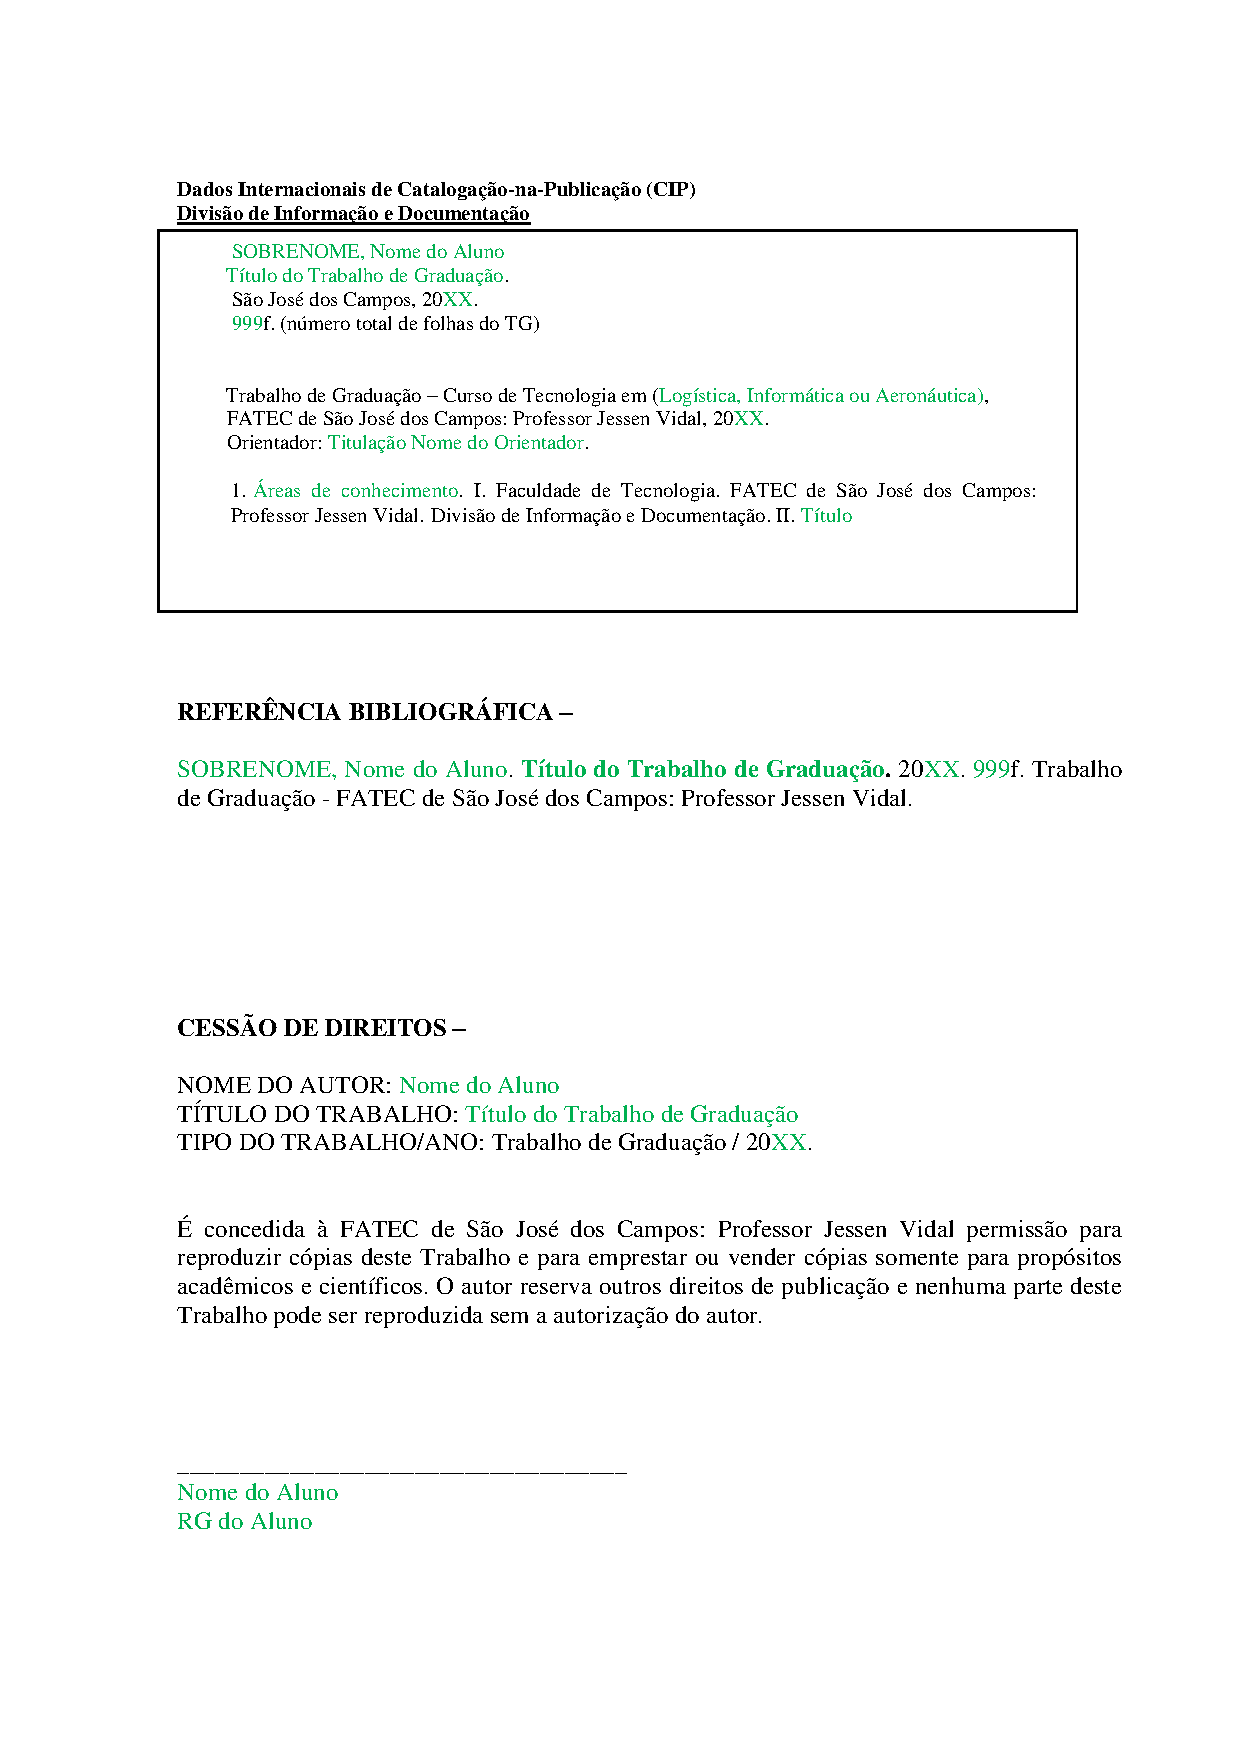
\includepdf{./testFicha}
    %%%%%%%%%%%%%
%
% Do not Edit this file!
%
%%%%%%%%%%%%%

\noindent\textbf{Dados Internacionais de Catalogação-na-Publicação (CIP)\\
Divisão de Informação e Documentação}

%\noindent\minibox[frame]{%
%    \indent INOUE, Marcos Hideki \\
%    \indent \imprimirtitulo \\
%    \indent \imprimirlocal, \the\year \\
%    \indent \pageref{LastPage}f. \\
%    \\ \\
%    \indent \imprimirtipotrabalho \-m \cursoRef \\
%    \indent \instituicaoRef, \the\year \\
%    \indent Orientador: \imprimirorientador \\
%    \indent Coorientador: \imprimircoorientador \\
%    \\
%    \indent \'Areas de Conhecimento. I. Faculdade de Tecnologia. \instituicaoRef. Divis\~ao de Informa\c{c}\~ao e Documenta\c{c}\~ao. II. \imprimirtitulo.
%}%

\noindent\framebox[\textwidth]{%
  % horizonal margin: 10\unitlength
  \parbox{400\unitlength}{%
    \sobrenomeRef, \nomeRef \\
    \imprimirtitulo \\
    \imprimirlocal, \the\year \\
    \pageref{LastPage}f. \\
    \\ \\
    \imprimirtipotrabalho\ -- \cursoRef \\
    \instituicaoRef, \the\year \\
    Orientador: \imprimirorientador \\
    Coorientador: \imprimircoorientador \\
    \\
    \'Areas de Conhecimento. I. Faculdade de Tecnologia. \instituicaoRef. Divis\~ao de Informa\c{c}\~ao e Documenta\c{c}\~ao. II. \imprimirtitulo
  }%
}\\
\parbox{400\unitlength}{
\vspace*{2cm}

\textbf{REFER\^ENCIA BIBLIGR\'AFICA ---} \\ \\
\sobrenomeRef, \nomeRef. \imprimirtitulo \the\year. \pageref{LastPage}f. \imprimirtipotrabalho\ -- \instituicaoRef.

\vspace*{3cm}
\textbf{CESS\~AO DE DIREITOS ---}\\ \\
NOME DO AUTOR: \imprimirautor \\
T\'ITULO DO TRABALHO: \imprimirtitulo \\
TIPO DO TRABALHO/ANO: \imprimirtipotrabalho/\the\year \\

\vspace*{2cm}
É concedida à FATEC de São José dos Campos: Professor Jessen Vidal permissão para reproduzir cópias deste Trabalho e para emprestar ou vender cópias somente para propósitos acadêmicos e científicos. O autor reserva outros direitos de publicação e nenhuma parte deste Trabalho pode ser reproduzida sem a autorização do autor.\\

\vspace*{2cm}
\noindent\rule{7cm}{0.4pt}\\
\imprimirautor \\RG: \rgRef
}
\end{fichacatalografica}

% ---
% Folha de aprovação
% ---

% Descomentar para imprimir a folha
%\begin{folhadeaprovacao}

  \begin{center}
    {\ABNTEXchapterfont\large\imprimirautor}

    \vspace*{\fill}\vspace*{\fill}
    \begin{center}
      \ABNTEXchapterfont\bfseries\Large\imprimirtitulo
    \end{center}
    \vspace*{\fill}

    \hspace{.45\textwidth}
    \begin{minipage}{.5\textwidth}
        \imprimirpreambulo
    \end{minipage}%
    \vspace*{\fill}

    Composição da Banca
   \end{center}

   \assinatura{\textbf{\imprimirorientador} \\ Orientador\\}
   \begin{center}
   \assinatura{\textbf{Dr. Reinaldo Gen Ichiro Arakaki} \\ Professor Convidado\\\vspace*{0.5cm}}
   \assinatura{\textbf{William Antônio Siqueira} \\ Convidado externo\\\vspace*{0.5cm}}
   \assinatura{\textbf{Luan Rafael Castor Pinheiro} \\ Convidado Externo\\\vspace*{0.5cm}}

   %\assinatura{\textbf{Professor} \\ Convidado 4}
   % Adicionar \assinatura para inserir linha de assinatura dos professores convidados
\end{center}   
   \begin{center}
    \vspace*{0.5cm}
    {\large\imprimirlocal}
    \par
    {\large\imprimirdata}
    \vspace*{1cm}
  \end{center}

\end{folhadeaprovacao}

% Descomentar quando o arquivo folhaAprov.pdf estiver no diretorio raiz
%\includepdf[]{folhaAprov.pdf}
% ---

% ---
% Dedicatória
% ---
\begin{dedicatoria}
   \vspace*{\fill}
   \centering
   \noindent
   DEDICATORIA
	% ToDo: Inserir aqui uma frase de dedicatório   
   % \textit{Alguma dedicatoria; frase bonita; e entre outros}
   \vspace*{\fill}
\end{dedicatoria}
% ---

% ---
% Agradecimentos
% ---
\begin{agradecimentos}

\par Agradeço a toda a minha família por me ajudar e incentivar durante toda a jornada de desenvolvimento deste trabalho. Sem vocês, nada disso seria possível.
\par Agradeço a todos os professores da Faculdade de Tecnologia de São José dos Campos - Professor Jessen Vidal, em especial ao professor Me. Giuliano Bertoti por toda confiança em mim depositada, por todas as conversas e por me mostrar o fantástico mundo da Inteligência Artificial.
\par Agradeço ao pessoal do Laboratório de Instrumentação de Sistemas Aquáticos (LabISA), que nos últimos dois anos me ajudaram muito no entendimento de tópicos relacionados ao assunto.
\par Agradeço também aos colegas e amigos que contribuíram de alguma forma para a realização deste Trabalho, em especial: Carlos Neto, Felipe Carvalho, Mauricio Yassunaga e Weslei Luiz.

%\par Agradeça todos que estiveram contigo e que te apoiaram, como amigos, professores, parentes, colegas de trabalho e entre outros.
\end{agradecimentos}

% ---

% ---
% Epigrafe
% ---
\begin{epigrafe}
    \vspace*{\fill}
    \begin{flushright}
% Little easter egg. 
%        \textit{''Eu acredito que os HotDogs simbolizam uma filosofia muito profunda, \\
%                na qual todos nós poderíamos ter a oportunidade de observá-la e aprendê-la. \\
%                O pão pode significar tudo que dá a nossa base para a nossa vida. \\
%                E a salsicha pode simbolizar nós mesmos, ou um simples conceito ou coisa que surge de uma epifania.''\\
%                (Rodrigo Takeshi, 26 de Outubro de 2016)}

        \textit{“Se cheguei até aqui foi porque me apoiei no ombro de gigantes.”\\
        (Isaac Newton)}
    \end{flushright}
\end{epigrafe}

% ---

% ---
% RESUMOS
% ---
% resumo em português
\setlength{\absparsep}{18pt} % ajusta o espaçamento dos parágrafos do resumo
% --- resumo em português ---
\begin{resumo}
    % Apresentação concisa dos pontos relevantes do documento deve ser exposta no resumo. No presente caso o resumo será informativo, assim deverá ressaltar o objetivo, a metodologia, os resultados e as conclusões do documento. A ordem desses itens depende do tratamento que cada item recebe no documento original. O resumo deve ser composto por uma seqüência de frases concisas, afirmativas e não em enumeração de tópicos. Deve ser escrita em parágrafo único e espacejamento de 1,5. A primeira frase deve ser significativa, explicando o tema principal do documento. Deve-se usar o verbo na voz ativa e na terceira pessoa do singular. Quanto a sua extensão, o resumo deve possuir de 150 a 500 palavras.   
    \vspace{\onelineskip}
    \noindent
    \textbf{Palavras-chave}: % palavras chaves, resumo, português.
\end{resumo}

% resumo em inglês
\begin{resumo}[Abstract]
    \begin{otherlanguage*}{english}
        %O abstract é o resumo da obra em língua estrangeira, que basicamente segue o mesmo conceito e as mesmas regras que o texto em português. Recomenda-se que para o texto do abstract o autor traduza a versão do resumo em português e faça, se necessário, os ajustes referentes à conversão dos idiomas. É importante observar que o título e texto NÃO DEVEM estar em itálico.
	    \vspace{\onelineskip}
	    \noindent
	    \\
	    \textbf{Keywords}: % Keywords, abstract, english.
    \end{otherlanguage*}
\end{resumo}
% ---

% ---
% inserir lista de ilustrações
% ---
\pdfbookmark[0]{\listfigurename}{lof}
\listoffigures*
\cleardoublepage
% ---

% ---
% inserir lista de tabelas
% ---
\pdfbookmark[0]{\listtablename}{lot}
\listoftables*
\cleardoublepage
% ---

% ---
% inserir lista de abreviaturas e siglas
% ---
% Listas de Siglas utilizadas no TG
\begin{siglas}
	\item[RNA] \emph{Redes Neurais Artificiais}
	\item[PMC] \emph{Perceptron Multicamadas}
	\item[AM] \emph{Aprendizado de Máquina}
	\item[AP] \emph{Aprendizado Profundo}
	\item[TFJS] \emph{TensorFlow.js}
	\item[RNC] \emph{Rede Neural Convolucional}
	\item[IBGE] \emph{Instituto Brasileiro de Geografia e Estatística}
	\item[H5] \emph{Arquivo Hierárquico do Keras}
	\item[API] \emph{Application Programming Interface}
	\item[TA] \emph{Tecnologia assistiva}
	\item[RA] \emph{Recurso assistivo}
	\item[Libras] \emph{Língua Brasileira de Sinais}
	\item[Colab] \emph{Colaboratory}
	\item[GPU] \emph{Graphics Processing Unit}
\end{siglas}

% ---

% ---
% inserir lista de símbolos
% ---
%% Lista de simbolos utilizadas no TG
\begin{simbolos}
	\item 
  % \item[$ m^2 $] Metro quadrado
  % \item[GHz] Giga-hertz
  % \item[MHz] Mega-hertz
\end{simbolos}
% ---
% ---
% inserir o sumario
% ---
\pdfbookmark[0]{\contentsname}{toc}
\tableofcontents*
\cleardoublepage
% ---

% ----------------------------------------------------------
% ELEMENTOS TEXTUAIS
% ----------------------------------------------------------

\textual

\setcounter{page}{15}
% ---
% Incluindo Capitulo 1 - Introducao
% ---
% ----------------------------------------------------------
% Introdução (exemplo de capítulo sem numeração, mas presente no Sumário)
% ----------------------------------------------------------
\chapter[Introdução]{Introdução}
%\addcontentsline{toc}{chapter}{Introdução}
% ----------------------------------------------------------

% \par O trabalho é motivado pela necessidade / oportunidade de...
% \par Apresentar brevemente o problema para explicar a motiva\~c\~ao para o realizar.
% \par Recomendável a utilização de figuras e/ou tabelas.

Este capítulo demonstra a motivação para o desenvolvimento deste trabalho, os objetivos deste e a metodologia adotada.

\section{Motivação} % Problema
% Dica do Mineda: Colocar mais referências, gastar mesmo aqui.... Isto ajuda a fazer com que a importância do trabalho seja esclarecida.

% Esta motivação está dando a entender que o problema a ser resolvido é outro, NÂO, lembre-se que, objetivo é demonstrar que recursos assistivos criados com Deep Learning podem ser aplicados em tecnologias da WEB!!!! BOa

% Colocar também uma observação feita pelo Arakaki -> O que é caro ? O que é barato ?


% e a necessidade de importação \cite{ANDRIOLI2017}. Sendo que, o alto custo, é justificado principalmente pela necessidade da criação de equipamentos específicos para cada caso

% O alto custo, na maioria dos casos pode ser justificado pela necessidade de desenvolvimento e construção de equipamentos específicos cada cada caso, isto por 

% \par No Brasil, há uma grande dificuldade de acesso aos recursos de tecnologia assistiva, causadas por diversos fatores, a citar, o alto custo e a necessidade de importação \cite{ANDRIOLI2017}. O alto custo, na maioria dos casos pode ser justificado pela necessidade de desenvolvimento e construção de equipamentos específicos, o que acaba gerando um alto valor de compra.

% . A principal característica

% estas que deixam de lado as deficiências de lado e focam nas habilidades já presentes no indivíduo \cite{tve2016} para permit

% em suas habilidades \cite{tve2016} para permitir 

% \cite{tve2016}

% são as tecnologias assistivas, 

% \par Para serem independentes nem todos os deficientes precisam de algum auxílio, porém aqueles que necessitam utilizam 

% \par Uma das maneiras de permitir que deficientes sejam inclusos na sociedade e tenham uma vida autônoma é com a utilização de  recursos de tecnologias assistivas, estas aliadas a serviços de tecnologia assistiva. Isto porque, estes recursos assistivos deixam de lado a deficiência, e focam nas habilidades presentes no individuo.

% Neste âmbito surgem as tecnologias assistivas

% e todas estas pessoas necessitam de uma vida inclusiva e independente, não sendo impedidas de realizar suas atividades por conta de suas 

% E todas estas pessoas necessitam de uma vida independente e de inclusão (SARTORETTO; BERSCH, 2017).

% \par No Brasil, há uma grande dificuldade de acesso aos recursos de tecnologia assistiva, causadas por diversos fatores, a citar, o alto custo e a necessidade de importação \cite{ANDRIOLI2017}. O alto custo, na maioria dos casos pode ser justificado pela necessidade de desenvolvimento e construção de equipamentos específicos, o que acaba gerando um alto valor de compra.

% \textbf{SE EU FALAR DE RECURSOS ASSISTIVOS DE BAIXO CUSTO, O TRABALHO TERÁ DE BUSCAR INFORMAÇÕES SOBRE PREÇO....PENSE NISTO....}

% \textbf{AQUI SERÁ LEGAL FALAR SOBRE A GRANDE DIFICULDADE DE AQUISIÇÃO DE RECURSOS ASSISTIVOS, E MESMO SOBRE OS AVANÇOS QUE TEM SIDO FEITOS....}

% % Não sei no que isto implica
% \textbf{TALVEZ FALAR SOBRE A GRANDE QUANTIDADE DE TRABALHOS SOBRE RECURSOS ASSISTIVOS E MESMO ASSIM POUCA APLICAÇÃO... --> "TALVEZ" <--}

\par De acordo com o censo do IBGE, realizado em 2010, no Brasil, há cerca de 45 milhões de pessoas com algum tipo de deficiência e todas estas necessitam de uma vida independente e inclusiva, não sendo impedidas de realizar suas atividades por conta da deficiência.

\par Para uma parte deste público-alvo, a solução para a inclusão e independência são as tecnologias assistivas \cite{ANDRIOLI2017}, que através dos avanços tecnológicos criam possibilidades para as pessoas que possuem deficiência \cite{Bersch2017}. Este tipo de tecnologia deixa de lado as deficiências e foca apenas nas habilidades já presentes nos indivíduos \cite{tve2016}.

\par Porém no Brasil, mesmo com diferentes iniciativas surgindo ao longo dos anos \cite{Bersch2017} há uma grande dificuldade de acesso aos recursos de tecnologia assistiva \cite{ANDRIOLI2017}, causados por diversos fatores, a citar, o alto custo, por conta da grande necessidade da criação de equipamentos específicos para cada caso \cite{tve2016}, e também a necessidade de importação destes equipamentos \cite{ANDRIOLI2017}.

\par Por outro lado, tem-se técnicas de Aprendizado Profundo, que através da aplicação de redes neurais artificiais profundas, desde 2012 vem sendo apresentadas como o estado-da-arte para a solução dos mais diversos problemas, nos mais variados contextos \cite{Ponti2018, forbes2019}, isto ocorrendo principalmente por conta da alta capacidade de generalização e adaptabilidade destes algoritmos \cite{Camila2017, Ponti2018, forbes2019}.

\par Estas características fizeram com que a procura e aplicação destes algoritmos aumentasse exponencialmente, como pode ser visto na Figura \ref{figure:interesse_aprendizado_profundo}. Isto fez com que diversas empresas como Google e Facebook começassem a utilizar muito destas técnicas em seus sistemas e aplicações, o que impulsionou a área de uma forma nunca antes vista.

\image{0.8}{intro/interesse_deep_learning.jpeg}{Interesse em aprendizado profundo de 2012 à 2019}{figure:interesse_aprendizado_profundo}{\citeonline{google2019}}

\par Com empresas interessadas na rápida prototipação e implementação destas técnicas em seus serviços, diversas bibliotecas de códigos, nas mais variadas linguagens, que facilitam a aplicação dessas técnicas foram criadas, e muitas disponibilizadas como \textit{software} livre. Dentre as bibliotecas disponibilizadas, destaca-se \cite{pytorch2017, tensorflowjs2019, tensorflow2015-whitepaper, chollet2015}. Estas bibliotecas trouxeram benefícios não apenas para as empresas por trás delas, mas também para todas as comunidades com interesse em tais técnicas.

\par Para a área cientifica, veio a oportunidade de aplicação de tais técnicas para impulsionar diferentes estudos como em \cite{Frid-Adar2018, Caroline2016}, e também outras empresas se beneficiaram expandindo seus negócios e áreas de atuação.

\par Neste contexto, para o desenvolvimento de recursos assistivos mais precisos e acessivos, as técnicas de Aprendizado Profundo começaram a ser aplicadas, como é o caso de \citeonline{Magalh2018}, que desenvolve um reconhecedor de gestos de Libras estado-da-arte com tais técnicas. Mas, estas aplicações ainda estão muito restritas apenas ao desenvolvimento e geração de modelos de redes neurais profundas, fazendo com que seja necessário a implementação destes em sistemas assistivos, como a biblioteca de navegação apresentada por \cite{handsfree2019}. Assim, este trabalho é motivado pela possibilidade do desenvolvimento de recursos assistivos para páginas da \textit{web} aplicando técnicas de Aprendizado Profundo, trazendo mais precisão as ferramentas desenvolvidas e mais acessibilidade para as páginas da \textit{web}.

% \cite{handsfree2019}

% , destacando principalmente a alta personalização destes algoritmos 


% com multiplicas camadas, que desde 2012

% que desde 2012 tem crescido exponencialmente (Figura \ref{})



% que são atualmente o estado-da-arte da solução de problemas com aprendizado de máquina.

% \cite{forbes2019}.

% \par Por outro lado, tem-se técnicas de \textit{Deep Learning}, que são atualmente o estado-da-arte da solução de problemas com aprendizado de máquina (PONTI, 2017), \textbf{DIVERSOS MERCADOS DE APLICAÇÃO...} isto por conta da grande capacidade de generalização diante de diferentes conjuntos de dados. Um de seus grandes benefícios é a possibilidade de alta personalização frente a diferentes tipos de usuários e aplicações.

% \par Desta forma, este trabalho foi motivado pela possibilidade da realização de um estudo de casos, onde técnicas de \textit{Deep Learning} são aplicadas para possibilitar a criação de recursos de tecnologias assistivas de baixo custo.

% \textbf{OS TEXTOS ABAIXO DEVEM SER TRANSFORMADOS EM CONTEÚDO}


% \textbf{DESDE 2012, COM A COMPETIÇÃO IMAGENET VENCIDA POR UM ALGORITMO DE DEEP LEARNING, AS COISAS PARA ESTA ÁREA APENAS MUDOU, TENDO O SURGIMENTO DE DIVERSAS BIBLIOTECAS (TENSORFLOW, KERAS, PYTORCH, TFJS, caffe <- Todos estes podem ser citados!!!}



% \textbf{ASSIM, DIVERSAS APLICAÇÕES COMEÇARAM A SER REALIZADAS COM DEEP LEARNING...}

% https://glitch.com/edit/#!/handsfree-starter?path=README.md:1:0
% http://www.each.usp.br/petsi/jornal/?p=1496
% http://www.acessibilidadelegal.com/20-padroes.php

% Section Objetivo Geral!
\section{Objetivo Geral}

\par O objetivo geral deste trabalho é desenvolver uma biblioteca JavaScript que possa levar recursos assistivos desenvolvidos através de técnicas de Aprendizado Profundo para páginas da \textit{web}.

% \par Implementar recursos de tecnologias assistivas de baixo custo, para usuários com deficiências auditiva e motora, utilizando técnicas de \textit{Deep Learning}

% Section Objetivo Especifico!
\section{Objetivo Espec\'ifico}

\par Para a consecução do objetivo geral foram estabelecidos os seguintes objetivos específicos:

\begin{itemize}
    \item Desenvolvimento de um recurso assistivo que permite a movimentação do \textit{cursor} do \textit{mouse} em páginas \textit{web} através de gestos da cabeça;
    \item Desenvolvimento de um recurso assistivo que permite a escrita de texto em campos de páginas da \textit{web} através de gestos de Libras;
    \item Integração das ferramentas desenvolvidas em uma biblioteca JavaScript.
\end{itemize}

\section{Metodologia} % COMO !! 
% Reescrever a metodologia (24/03/2019)

\par A realização dos objetivos específicos deste trabalho são feitas através da aplicação de modelos de Aprendizado Profundo no desenvolvimento dos recursos assistivos para páginas da \textit{web}, todos estes consolidados através de uma biblioteca JavaScript.

\par Para o desenvolvimento do recurso assistivo de escrita de texto com gestos de Libras, dados serão coletados e um modelo MobileNet \cite{howard2017mobilenets} será treinado com os dados para possibilitar o reconhecimento de gestos e então traduzir estes para textos. Já no recurso assistivo para a movimentação do \textit{mouse}, através da aplicação do modelo PoseNet \cite{PoseNetMedium2019}, junto a regressões lineares, será feito o mapeamento dos gestos do usuário para posições do \textit{mouse} na tela.

\par A disponibilização e utilização destes modelos dentro da biblioteca desenvolvida neste trabalho, esta nomeada de ICan.js, será feita através de módulo Tensorflow para JavaScript \cite{tensorflowjs2019}.

% A realização dos objetivos específicos do trabalho é feita através da aplicação de modelos de DL no desenvolvimento das ferramentas. A linguagem de programação empregrada para o desenvolvimento das ferramentas é o Javascript, junto ao \textit{framework} de desenvolvimento de DL \textit{Tensorflow.js}

% Por contar com diferentes estudos de caso, todas as ferramentas são desenvolvidas de maneira modular, a permitir que, no momento da integração entre as ferramentas desenvolvidas, injeções de dependências sejam realizadas para tal.

% Cada uma das ferramentas desenvolvidas, faz a utilização de um modelo de DL, no caso do controle do \textit{mouse} o modelo Posenet (KENDALL, 2015) é utilizado, para facilitar a identificação de pontos faciais do usuário, e permitir que cada gesto seja mapeado em movimentos do \textit{mouse}, o reconhecimento de voz, por sua vez, é feito com o \textit{Web Speech API}, uma \textit{API} livre que facilita a sintetização de som em texto. Por fim, para a tradução de LIBRAS em texto, será utilizado uma rede neural convolucional (LECUN et al, 1998), que apresenta bons resultados na classificação de imagens, junto a um conjunto de imagens de LIBRAS criado pelo autor.

% Retirado apenas para ganhar tempo! <- Esta ainda é a oficial e deve ser levada em consideração ! ! !
% o retreino do modelo de rede neural Mobilenet (HOWARD, A; WANG, W, 2017) é feito, permitindo que, mesmo com poucas imagens, a rede neural possa convergir na classificação dos sinais de LIBRAS.

\section{Organização do trabalho}

Este Trabalho está organizado nos seguintes capítulos:

\begin{itemize}
    \item 2 - Fundamentação Teórica
    \par O capítulo expõe os conceitos necessários para a compreensão do presente trabalho.
    \item 3 - Desenvolvimento
    \par Este capítulo aborda detalhadamente a especificação da biblioteca JavaScript, assim como a metodologia empregada para o desenvolvimento de cada um dos recursos assistivos.
    \item 4 - Resultados
    \par Neste capítulo são expostos, através de aplicações de exemplo, os resultados alcançados com a metodologia aplicada na implementação dos recursos assistivos e na biblioteca.
    \item 5 - Considerações Finais
    \par Este capítulo apresenta as conclusões obtidas com os resultados, assim como uma breve sugestão de trabalhos futuros.
\end{itemize}

% 	\item Capítulo 2: Revisão bibliográfica
% 	\item Capítulo 3: Desenvolvimento % mostra a implementação das tecnologias assistivas com Deep Learning;
% 	\item Capítulo 4: Resultados % expõe os resultados;
% 	\item Capítulo 5: Considerações finais % apresenta as considerações finais
% \end{itemize}


% ---

% ---
% Incluindo Capitulo 2 - Fundamentacao Teorica
\chapter{Fundamentação Teórica}
\label{ch:fundamentacao}
\par Neste capítulo ser\~ao fundamentados os conhecimentos b\'asicos para o entendimento do trabalho.

\section{Tecnologias assistivas}

\textbf{ESTA SUBSEÇÃO AINDA SERÁ ESCRITA}

% \section{Deficiência} % Este título está completamente problemático....
% 07/03/2019 -> O Giuliano disse que isto pode ser mantido sem problemas...
% Vou reestruturar o capítulo e então colocar mais referências...

% \par De acordo com o censo do IBGE, realizado em 2010, cerca de 6.2\% da população brasileira possui algum tipo de deficiência. E a necessidade de inclusão destas pessoas na sociedade é extremamente importante. Do grupo citado anteriormente, cerca de 1.3\% tem algum tipo de deficiência auditiva, e 1.1\% tem deficiências auditivas

% \par Para aqueles com deficiência auditiva, a comunicação e inclusão pode ser feita através da Linguagem Brasileira de Sinais, segunda língua oficial do Brasil desde 2005. Mas, pode-se encontrar problemas com a comunicação através de LIBRAS principalmente pelo fato de, boa parte dos ouvintes não falar esta língua o que acarreta também na baixa utilização desta em diversos meios de comunicação. Um ponto importante apontado no documentário feito pela TVE RS, é que, pessoas com deficiência auditiva, normalmente são alfabetizadas somente com LIBRAS, por terem muita difículdade e falta de estrutura para o aprendizado da Língua Portuguesa. Ainda de acordo com o documentário, para as pessoas com deficiências motoras há os recursos de tecnologias assitivas, que aumentar a facilidade do acesso destas pessoas aos meios sociais, principalmente os digitais.

% Precisa ficar realizando definições de cada uma das deficiências que serão tratadas no trabalho ?? Pensando hoje, acho que deveria sim! 
%% Caso precise, qual o nível de profundidade necessário ? ? ? Não tão profundo, mas a ponto de demonstrar a qual público o trabalho é destinado

% \section{Tecnologias assistivas}

% NTAAI -> Verificar como citar esta fonte ! ! !
% Verificar se devo citar tecnologias assistivas, ou no meu caso, recursos assistivos ! ! !
% (13/03/2019) -> Veja que, será legal colocar tudo sobre as deficiências aqui... isto evita o título ofensivo acima..., e a coisa tem um foco mais interessante...
% \par Uma das formas de realizar a inclusão social de pessoas com deficiência é através da inclusão digital, utilizando técnologias assitivas, estes que visam ampliar as habilidades presentes no indivíduo, não o forçando a ter características específicas para a inclusão (NTAAI, 2016). As tecnologias assitivas, de acordo com o Núcleo de Tecnologia Assistiva, Acessibilidade e Inovação da Universidade de Brasilia, podem ser divididas em dois grupos, os recursos, que representam equipamentos que expandem as habilidades dos indivíduos com deficiência, e os serviços, que normalmente são aqueles relacionados a facilitação e capacitação para o uso correto dos recursos assistivos.

% Adicionar dados aqui que fazem jus ao que estou dizendo ! ! !
% Paragrafo abaixo deve antes ser reescrito para o novo escodo do trabalho
% Para aqueles que possuem deficiência motora, a inclusão digital vem através de \textit{mouses} adaptados, formas diferentes de utilizar teclados, ou até mesmo a utilização do computador por comandos de voz. E para os surdos ferramentas que ajudam no processo de interação já levando em consideração problemas com a alfabetização.


%%%%%%%%%%%%%%%%%%% Temporário (Coloquei aqui pois utilizo no trabalho, mas vou falar com o Giuliano)
% \section{Regressões}
% \par Um pequeno descritivo sobre regressões
%%%%%%%%%%%%%%%%%%%

%%% 17/02/2019
% Verificar o que pode ser feito com a análise de regressão
% Vendo o que o Felipinho disse, realmente parece que a regressão está foram do lugar aqui
%%%
% \section{Análise de Regressão} % Ou Regressão linear

% MACHADO -> https://www.ime.usp.br/~fmachado/MAE229/AULA10.pdf
% PETERNELLI -> http://www.dpi.ufv.br/~peternelli/inf162.www.16032004/materiais/CAPITULO9.pdf
%A análise de regressão estuda a relação entre uma variável dependente e outras independentes (MACHADO, 2015). Esta relação é representada através de um modelo matemático (MACHADO, 2015), este que pode ter diferentes formas sendo linear, quadrático, exponencial entre outros (PETERNELLI, 2003). 

% ToDo: Colocar um exemplo ? Se for colocar, qual será ? (02/02/2019)

%%%%%%%%%%%%%
% Antiga definição utilizada: Análise de regressão consiste na aplição de uma análise estatística com o objetivo de verificar a relação entre duas variáveis (PETERNELLI, 2003).
% Aqui eu posso colocar assim: Neste trabalho, após a verificação dos dados fez-se a utilização de regressões lineares
% Claro que isto deverá ser reescrito, até porque coloquei com as minhas palavras
% \par Os métodos de regressão são aqueles que buscam através de variáveis continuas ou categóricas estimar uma outra variável, podendo esta também ser continua ou categórica. Para este trabalho utilizou-se do método de regressão linear, este que básicamente busca através de uma função f(x) mapear a relação de duas variáveis linearmente separáveis.
%%%%%%%%%%%%%

% \section{Correlação de imagens digitais}

% http://www.dpi.inpe.br/~carlos/Academicos/Cursos/Pdi/pdi_estatisticas.html
% Se tudo funcionar da forma que estou pensando, vou colocar este conceito aqui (02/02/2019)
% Pois bem, não funcionou como eu esperada, assim vou manter este conceito de fora do documento (03/02/2019)

% \par A correlação é A, porém para este trabalho ela foi empregada em Imagens digitais

% \subsection{Regressão logistica}

% \par Uma função que divide o espaço, porém levando em consideração variáveis dependentes categóricas
%%%%%%%%%%%%%%%%%%%

\section{Inteligência artificial}

%%%%%%%%%%%%%%%%%%%%% Verificar a necessidade de escrever sobre inteligência artificial ! ! ! No momento (01/02/2019) eu acho que devo escrever sobre

% Rever todas as referências - Provavelmente reescrever o texto nas férias ! ! ! (Já arrumei melhor as coisas neste capítulo (01/02/2019)
% Von Zuben: ftp://ftp.dca.fee.unicamp.br/pub/docs/vonzuben/ea072_2s13/introducao_EA072_2s2013.pdf
% (Winston, 1992) Livro do Winston

\par Sistemas inteligentes de forma geral são aqueles que apresentam a capacidade de planejar e resolver problemas através de dedução e indução utilizando conhecimentos de situações anteriores \cite{VonZuben2013}, e a inteligência artificial, é um campo da ciência e engenharia de computação \cite{VonZuben2013}, que possibilitam a sistemas computacionais, perceber, raciocionar e agir \cite{Winston1992}.

% Augusto -> http://dcm.ffclrp.usp.br/~augusto/teaching/ami/AM-I-Conceitos-Definicoes.pdf
\par As técnicas computacionais mais utilizadas para o desenvolvimento e aplicação de inteligência artificial, são aquelas relacionadas ao aprendizado de máquina. Esta que é uma área que tem como objetivo principal, desenvolver técnicas que permitam aos sistemas adquirir conhecimento de forma automática e com estes conhecimentos tomar decisões \cite{Augusto2007}.

% NG -> Curso do andrew
\par Para a realização do aprendizado de máquina, existem diversas técnicas, que vão de simples regressões estatísticas, até modelos complexos, como às redes neurais artificiais (RNA) (NG, 2016).
%%%%%%%%%%%%%%%%%%%%%

\section{Redes neurais artificiais}

% Colocar mais referências em redes neurais artificiais, exemplos de uso.... acho que fica legal
% Haikin (2001) -> Livro (Redes Neurais: Princípios e Prática)
% Cintra -> Minicurso do INPE (2015)

% É um começo, mas ainda não estou feliz com o resultado.... (01/02/2019)
\par Redes neurais artificiais são sistemas computacionais que busca modelar o sistema cerebral natural humano, estas que são uma das formas de soluções de problemas apresentados dentro do âmbito de inteligência computacional \cite{Cintra2019}.

%% Não creio que isto esteja escrito da melhor forma, mas está melhor que o texto inicial (01/02/2019)
% Escrever mais!! Fale sobre machine learning aqui tbm -> As referências do Deep Learning with R são boas ! (13/03/2019)
\par Por buscar modelar o cérebro humano, as RNAs utilizam como unidade básica de processamento, os neurônios artificiais \cite{Haykin2001}, da mesma forma que o cérebro utiliza os neurônios biológicos. % Preciso criar um complemento para ir para o próximo capítulo ? (01/02/2019)

%Acho que esta segunda parte não está combinando com o resto do texto, mas por agora vou manter aqui
% Por buscar modelar o cérebro humano, a unidade básica de processamento das RNAs são os neurônios (HAYKIN, 2001), estruturas estas que tem fortes ligações com o sistema biológico.

%%%%%%% Partes antigos
% Redes neurais artificiais (RNA) são modelos criados para representar a maneira como o cérebro realiza suas tarefas, sendo estas maciçamente paralelas e distribuidas (HAYKIN, 2001). Ainda de acordo com Haykin (2001), estes modelos para ter bons desempenhos são representados normalmente através de interligações maciças de células computacionais simples, denominadas de neurônios. 
% Veja que, para a criação destes modelos, há uma grande inspiração em aspectos e funcionamentos do cérebro humano (CINTRA, 2015)
% Acho que isto aqui deve ser complementado ! ! ! Com toda a certeza!
% Cintra - Minicurso INPE (2015)
% Como descrito na seção anterior, uma das áreas de aplicação do aprendizado de máquina mais avançadas atualmente são as RNA, que imitam principalmente aspectos do funcionamento do corpo humano, neste caso, o cérebro e suas redes neuronais (CINTRA, 2015). 
%%%%%%%

\subsection{Neurônio biológico}

% Falar sobre sinapses ! ! ! -> Já falei sobre isto ! ! !
% Falar sobre como aprendemos ! ! ! -> Será  mesmo necessário ? ? ?

% Nunes -> Livro
\par Todo o processamento de informações no cérebro humano, é feito através de elementos biológicos de processamento, que operam em paralelo para a produção de ações apropriadas para cada estímulo recebido pelo corpo. A célula base do sistema nervoso cerebral é o neurônio (Figura \ref{figure:bioneuron}), e sua principal função é conduzir impulsos (Representando os estímulos) levando em consideração as condições do corpo e assim produzindo ações. Os neurônios também são os responsáveis pelos atos do pensamento e armazenamento de informações \cite{livroNunes2016}.

\par Os neurônios podem ser divididos em três partes elementares, os dendritos, que captam de forma continua os impulsos vindos de outros neurônios, o corpo celular, que processa todas as informações captadas e os axônios que enviam as informações processadas no corpo celular para outros neurônios.

% https://www.researchgate.net/figure/Figura-24-Ilustrativo-de-um-neuronio-biologico_fig17_303369695
\image{1.4}{neuronio-biologico.png}{Ilustração do neurônio biológico}{figure:bioneuron}{\citeonline{Remes2016}}

% SHEPERD -> Artigo
% XAVIER -> Artigo (Divulgado no Alô Ciência) !
% Consultar o livro do Hebb apenas para ter uma certeza!
\par Estima-se que a rede neural cerebral, possui cerca de 100 bilhões de neurônios, cada um destes mantendo conexão com uma média de 6.000 outros neurônios, gerando cerca de 600 trilhões de conexões (SHEPHERD, 1990). A região de conexão entre os neurônios são chamadas de sinapses, estas que como apresentado por Donald Hebb em 1949, em seu livro \textit{The Organization of Behavior} são fortalecidas todas as vezes em que são utilizadas.

% A regiã entre os neurônios são chamados de sinapses, estas que como apresentado por Donald Hebb em 1949, em seu livro \textit{The Organization of Behavior} tem os caminhos fortalecidos toda vez que é utilizado
% , assim, pode-se entender que, neurônios tem propensões para certas atividades, quando os neurônios utilizados por esta tem suas sinapses bem fortalecidas (XAVIER, 2017).

\par A Figura \ref{figure:nncotex} demonstra um exemplo de uma pequena parte das redes neuronais responsáveis pelo córtex auditivo.

% ToDo
% https://pt.wikipedia.org/wiki/Ficheiro:Cajal_actx_inter.jpg
% MAnter wikipédia é foda...
\image{0.35}{nn_cortex.jpg}{Rede neural do córtex auditivo}{figure:nncotex}{}

%%% Validar as informações abaixo
% Citar assim Hodgkin e Huxley (1952) ou (Hodgkin; Huxley, 1952) ? ? ?

% McCulloch -> Artigo
% (HODGKIn, HUXLEY, 1952) ? ? ? 
\par A representação inicial deste conjunto de neurônios em sistemas de computação foram implementadas através de circuitos eletrônicos, com apresentado por McCulloc e Pitts (1943), estes que foram utilizados como base para a criação dos modelos de neurônios artificiais apresentados por Hodgkin e Huxley (1952).
%%%

\subsection{Neurônio artificial}

\par Como citado anteriormente, os neurônios artificiais, são modelos computacionais para a representação do neurônio biológico nas RNAs, e da mesma forma que em um neurônio biológico, a representação deste é feita com três elementos básicos \cite{Haykin2001}:  

\begin{itemize}
	% Posso colocar Conjunto de sinapses, representado por Xn... ? (02/02/2019)
	\item Conjunto de sinapses, cada uma caracterizada por um peso, este que indica a relevância de cada valor de entrada;
	\item Somador, ou combinador linear, que faz a ponderação dos valores de entrada com as respectivas sinapses do neurônio;
	\item Função de ativação utilizada para restringir os valores de saída do neurônio.
\end{itemize}

\par Ainda de acordo com \citeonline{Haykin2001}, a estes modelos neuronais pode-se aplicar um \textit{bias}, este que será o responsável pelo aumento ou diminuição dos valores de entrada da função de ativação. Em termos matemáticos, pode-se descrever um neurônio k (Figura \ref{figure:nn_mcculloch}) com as seguintes equações \cite{Haykin2001}:

\begin{equation}
	u_{k} = \sum_{j=1}^{n} w_{kj} x_{j}
\end{equation}
e
\begin{equation}
	y_{k} = f(u_{k} + b_{k})	
\end{equation}
onde $ x_{1}, x_{2}, ..., x_{n} $ são os sinais de entrada; $ w_{k1}, w_{k2}, ..., w_{kn} $ são os pesos sinápticos do neurônio k; $ u_{k} $ é a saída do combinador linear; $ b_{k} $ é o \textit{bias}; $ f(u_{k} + b_{k}) $ a função de ativação; e $ y_{k} $ representa a saída do neurônio.

% Os neurônios artificias, que são modelos de representações dos neurônios biológicos compoem a RNA. O principal modelo de neurônio artificial utilizado, mesmo em arquiteturas mais atuais, é o proposto por McCulloch e Pitts em 1943 (Figura 3). Neste há componentes que fazem referência direta ao neurônio biológico visto anteriormente.

% Imagem adaptada de Haykin (2001)
% \image{0.1}{nn_mculloch.jpg}{Modelo de Neurônio artificial}{figure:nn_mcculloch}{Adaptado de \cite{Haykin2001}}
\begin{figure}[H]
    \centering
   \begin{tikzpicture}[
init/.style={
  draw,
  circle,
  inner sep=2pt,
  font=\Huge,
  join = by -latex
},
init2/.style={
  draw,
  circle,
  inner sep=2pt
},
neuron missing/.style={
    draw=none, 
    scale=4,
    text height=0.333cm,
    execute at begin node=\color{black}$\vdots$
  },
squa/.style={
  draw,
  inner sep=2pt,
  font=\Large,
  join = by -latex
},
squa2/.style={
  draw,
  inner sep=2pt,
  font=\Large
},
start chain=2,node distance=13mm
]
\node[on chain=2] 
  (x2) {$x_2$};
%\node[below of=x2] (dots) {$\vdots$} -- (dots) node[right of=dots] (ldots) {$\vdots$};
%\node[below of=2] (dots) {$\vdots$} -- (dots) node[left of=dots] (ldots) {$\vdots$};
\node[on chain=2,init2,join=by o-latex] 
  {$w_{k2}$};
\node[on chain=2,init] (sigma)
  {$\displaystyle\Sigma$};
\node[on chain=2,squa2,label=above:{\parbox{2cm}{\centering Função de \\ ativação}}](te) {$f$};
\node[on chain=2,label=above:Saída] (sa)
  {$y_k$};
\begin{scope}[start chain=1]
\node[on chain=1] at (0,1.5cm) 
  (x1) {$x_1$};
\node[on chain=1,init2,join=by o-latex] 
  (w1) {$w_{k1}$};
\end{scope}
\begin{scope}[start chain=3]
\node[on chain=3] at (0,-1.5cm) 
  (x3) {$x_n$};
\node[on chain=3, init2,label=below:{\parbox{2cm}{\centering Pesos \\ sinápticos}},join=by o-latex] 
  (w3) {$w_{kn}$};
\end{scope}
\node[label=above:\parbox{2cm}{\centering Bias \\ $b$}] at (sigma|-w1) (b) {};

\draw[-latex] (w1) -- (sigma);
\draw[-latex] (w3) -- (sigma);
\draw[o-latex] (b) -- (sigma);
\draw[-latex] (sigma) -- (te) node[midway,sloped, above]{$v_k$};
\draw[-latex] (te) -- (sa) node[midway,sloped, above]{};
\draw[decorate,decoration={brace,mirror}] (x1.north west) -- node[left=10pt] {Entradas} (x3.south west);
\end{tikzpicture}
    \caption{Neurônio Artificial}
    \fonte{Adaptado de \citeonline{Haykin2001}}
    \label{fig:modelo_neuronio}
\end{figure}

\par A partir da Figura 3 é possível realizar uma comparação entre cada um dos elementos do neurônio artificial e biológico. Os sinais de entrada, advindos do meio externo, normalmente uma aplicação, são análogos aos impulsos elétricos captados pelos dendritos no neurônio biológico.  Os pesos sinápticos representam a importância do sinal recebido para o neurônio, o que representa as ponderações exercidas pelas junções sinápticas do modelo biológico, ou seja, a força do caminho entre as sinapses, citados anteriormente. O campo de somatório junto a função de ativação, representam o corpo celular do neurônio biológico, é nesta parte que os resultados criados pelo neurônio são calculados \cite{livroNunes2016} 

\subsection{Arquiteturas de rede} 

\par Para \citeonline{livroNunes2016} uma RNA pode ser constituída de até três partes diferentes, estas denominadas de camadas, as quais são nomeadas a seguir:

\begin{itemize}
    \item Camada de entrada: É a camada responsável pelo recebimento de dados;
    \item Camadas escondidas, intermediárias ou ocultas: São camadas compostas de neurônios responsáveis pela extração de características associadas ao processo ou sistema;
    \item Camadas de saída: Também constituída de neurônios, esta camada é responsável pela produção e apresentação dos resultados finais da rede.
\end{itemize}

\par Das camadas descritas acima, devem estar presentes em uma RNA no mínimo a camada de entrada e a camada de saída \cite{Cintra2019}.

\par Diferentes formas de organização de cada uma destas camadas, especialmente relacionadas a forma de relação entre os neurônios, definem as arquiteturas de RNA \cite{livroNunes2016}. \citeonline{Haykin2001} define a existência de duas classes de arquiteturas fundamentais, sendo elas: Redes de alimentação direta, com uma ou várias camadas e Redes recorrentes.

\par As redes de alimentação direta, são denominadas desta forma por conta de seu fluxo percorrer uma única direção \cite{Cintra2019}, iniciando o fluxo na camada de entrada seguindo pelas diferentes camadas até o neurônio de saída. Este tipo de rede pode possuir uma ou várias camadas ocultas.

% Verificar se devo abreviar a sigla de redes de alimentação direta.... (04/03/2019)
\par Para as redes de alimentação direta com uma única camada, tem-se como tipo comum a \textit{Perceptron} (Figura \ref{figure:camadaunida}). Em sua estrutura são apresentadas duas camadas, entrada e saída, porém são nomeadas de camada única já que existem operações matemáticas ocorrendo apenas na camada de saída \cite{livroNunes2016}.

\begin{figure}[H]
    \centering
    \def\layersep{2.5cm}
\begin{tikzpicture}[shorten >=1pt,->,draw=black!50, node distance=\layersep]
    \tikzstyle{every pin edge}=[<-,shorten <=1pt]
    \tikzstyle{neuron}=[circle,fill=black!25,minimum size=17pt,inner sep=0pt]
    \tikzstyle{input neuron}=[neuron, fill=black!50];
    \tikzstyle{output neuron}=[neuron, fill=black!50];
    \tikzstyle{hidden neuron}=[neuron, fill=black!50];
    \tikzstyle{annot} = [text width=4em, text centered]
    \tikzset{normal arrow/.style={draw,-triangle 45,very thick}}

    % Draw the input layer nodes
    \foreach \name / \y in {1,...,4}
    % This is the same as writing \foreach \name / \y in {1/1,2/2,3/3,4/4}
        \node[input neuron, pin=left:Entrada $x$$_\y$] (I-\name) at (0,-\y) {};

    % Draw the hidden layer nodes
    \foreach \name / \y in {1,...,5}
        \path[yshift=0.5cm]
            node[hidden neuron] (H-\name) at (\layersep,-\y cm) {};

    % Draw the output layer node
    %\node[output neuron,pin={[pin edge={->}]right:Saída}, right of=H-3] (O) {};

    % Connect every node in the input layer with every node in the
    % hidden layer.
    \foreach \source in {1,...,4}
        \foreach \dest in {1,...,5}
            \path (I-\source) edge (H-\dest);
            

    % Connect every node in the hidden layer with the output layer
    \foreach \source in {1,...,5}
        \draw[->] (H-\source) -- +(0.9,0);
        %\path (H-\source)  -- ();
        %\draw [->] (0,0) -- (30:20pt); 

    % Annotate the layers
    \node[annot,above of=H-1, node distance=1.5cm] (hl) {Camada de \\ Saída};
    \node[annot,left of=hl] {Camada de entrada};
    %\node[annot,right of=hl] {Camada de saída};
\end{tikzpicture}
    \caption{Rede de alimentação direta de camada única}
    \fonte{Adaptado de \citeonline{livroNunes2016}}
    \label{figure:camadaunida}
\end{figure}

% Novamente, dúvidas nas siglas... (04/03/2019)
% Referenciar este parâgrafo.... escrevendo apenas para montar a ideia e já completar a doc....
% Figura XY -> Imagem 
\par Já as redes de alimentação direta com múltiplas camadas (Figura \ref{figure:multilayer_perc}), diferentes das redes de camada única, possuem diversas camadas ocultas. Para esta classe o tipo mais comum são as Perceptron multicamadas (do inglês \textit{Multilayer Perceptron} - MLP), estas que por possuírem mais camadas são capazes de extrair quantidades maiores de características do problema que está sendo modelado pela rede.

\begin{figure}[H]
    \centering
    \def\layersep{2.5cm}

\begin{tikzpicture}[shorten >=1pt,->,draw=black!50, node distance=\layersep]
    \tikzstyle{every pin edge}=[<-,shorten <=1pt]
    \tikzstyle{neuron}=[circle,fill=black!25,minimum size=17pt,inner sep=0pt]
    \tikzstyle{input neuron}=[neuron, fill=black!50];
    \tikzstyle{output neuron}=[neuron, fill=black!50];
    \tikzstyle{hidden neuron}=[neuron, fill=black!50];
    \tikzstyle{annot} = [text width=4em, text centered]

    % Draw the input layer nodes
    \foreach \name / \y in {1,...,4}
    % This is the same as writing \foreach \name / \y in {1/1,2/2,3/3,4/4}
        \node[input neuron, pin=left:Entrada $x$$_\y$] (I-\name) at (0,-\y) {};

    % Draw the hidden layer nodes
    \foreach \name / \y in {1,...,4}
        \path[yshift=0cm]
            node[hidden neuron] (H-\name) at (\layersep,-\y cm) {};
            
    % Draw the second hidden layer nodes
    \foreach \name / \y in {1,...,5}
        \path[yshift=0.5cm, xshift=1.9cm ]
            node[hidden neuron] (J-\name) at (\layersep,-\y cm) {};

    % Draw the output layer node
    \node[output neuron,pin={[pin edge={->}]right:Saída}, right of=J-3] (O) {};

    % Connect every node in the input layer with every node in the
    % hidden layer.
    \foreach \source in {1,...,4}
        \foreach \dest in {1,...,4}
            \path (I-\source) edge (H-\dest);
   
   % Connect every node in the hidden layer 1 with every node in the
    % hidden layer 2.     
     \foreach \source in {1,...,4}
        \foreach \dest in {1,...,5}
            \path (H-\source) edge (J-\dest);

    % Connect every node in the hidden layer with the output layer
    \foreach \source in {1,...,5}
        \path (J-\source) edge (O);

    % Annotate the layers
    \node[annot,above of=H-1, node distance=1.5cm] (hl) {1º Camada \\ oculta};
    \node[annot,above of=J-1, node distance=1.5cm] (hl2) {2º Camada \\ oculta};
    \node[annot,left of=hl] {Camada de entrada};
    \node[annot,right of=hl2] {Camada de \\ saída};
    %\node[annot,above of=H-1, node distance=1.5cm] (hl) {Camada de \\ Saída};
\end{tikzpicture}
    \caption{Rede de múltiplas camadas}
    \fonte{Adaptado de \citeonline{livroNunes2016}}
    \label{figure:multilayer_perc}
\end{figure}

\par Por fim as redes recorrentes, que recebem este nome por conta da realimentação entre os neurônios da mesma camada, ou seja, a saída de um neurônio em uma camada, pode servir como entrada para outro neurônio da mesma camada \cite{Nelson2017}.

\par Estas formas de organização presentes nas arquiteturas, estão intimamente relacionadas ao processo de aprendizado que é aplicado nas RNAs \cite{Haykin2001}.

\subsection{Processo de aprendizado}

\par Um dos pontos mais relevantes das RNAs é a generalização \cite{livroNunes2016}, onde treina-se levando em consideração um conjunto amostral \textit{A}, este que faz uma boa representação do problema resolvido na tarefa (REF), e então após este processo a rede consegue realizar a tarefa não somente para o conjunto \textit{A}, mas também para um conjunto \textit{C} qualquer \cite{livroNunes2016}.

\par Porém para a generalização, como citado, é necessário um processo de treinamento, este que seja adequado a arquitetura de rede neural. \citeonline{livroNunes2016} definem processo de treinamento como um algoritmo que, através de seus passos bem definidos ajusta os pesos sinápticos da rede com o objetivo de permitir o mapeamento das relações dos dados e então realizar o processo de generalização. 

\par Os processos de treinamento podem adotar diferentes estratégias para ensinar as RNAs, e cada estratégia gera um algorítimo de aprendizado diferente, sendo os principais, os algorítimos de aprendizado supervisionado e não-supervisionado.

% Inserir aqui a explicação da divisão dos dados entre treino e teste....Uma pequena descrição é o suficiente.
\par No aprendizado supervisionado, há rótulos $y^{(t)}$ que indicam o comportamento $\widehat{y}$ que a rede deve apresentar para cada $x^{(t)}$ presente em um conjunto de dados $\{(x^{(t)}, y^{(t)}): 1 \leqslant t \leqslant T\}$ \cite{bezerra2016}. Desta forma, de acordo com os resultados apresentados, ajustes são feitos nos pesos sinápticos e limiares dos neurônios da rede \cite{livroNunes2016}, com o objetivo de fazer com que a saída da rede seja o mais próximo possível de $y^{(t)}$ \cite{Osorio1999}. Já o aprendizado não supervisionado, são utilizados apenas os dados, sem qualquer tipo de rótulo e sua intenção é realizar agrupamentos \cite{Camila2017}, levando em consideração características relevantes, estas identificadas pela rede.

\par Após a aplicação dos algoritmos de treinamento é necessário avaliar a performance do modelo de RNA gerado, para garantir que o mesmo está sendo capaz de generalizar.

\par Uma maneira de realizar esta avaliação é verificando a acurácia da RNA, esta que é calculada medindo a quantidade de acertos do modelo frente a um conjunto de dados não visto durante o processo de treinamento, por isto em diversos casos o conjunto de dados é dividido em dados de treino e teste \cite{Goodfellow-et-al-2016}.

\par A separação dos dados, pode ser utilizada também para a identificação de problemas de \textit{Underfitting}, que é causado quando o modelo não consegue extrair características relevantes do conjunto de dados, obtendo altas taxas de erro durante o treinamento, ou mesmo o \textit{Overfitting}, que ocorre quando o modelo extrair características além do necessário do conjunto de dados, fazendo assim com que o modelo tenha baixas taxas de erro no treino e praticamente não acerte no teste. \cite{Goodfellow-et-al-2016}.

% No aprendizado supervisionado, é considerado adisponibilidade de um conjunto de treinamento  é o vetor de características que está associado ao componente $y^{t}$ \cite{bezerra2016}, e então, para cada $x^{t}$ a rede gera um componente resultante $\widehat{y}$, este que será utilizado  

% NG -> Neste caso é o curso do Andrew NG
% No aprendizado supervisionado, o usuário indica o comportamento que a RNA deve apresentar dado um conjunto de dados qualquer, desta forma, a RNA pode ir ajustando os pesos sinápticos de seus neurônios com o objetivo de produzir o mesmo resultado apresentado pelo usuário. Já o aprendizado não supervisionado, oposto do supervisionado, é apresentado para a RNA apenas o conjunto de dados, e a RNA se encarrega de aprender sobre aquele conjunto de dados. Este tipo de aprendizado pode ser utilizado para deixar a RNA identificar os padrões presentes nos dados, e tirar informações destes padrões (NG, 2013). 

% \subsubsection{Transferência de aprendizado}
% Isto aqui está completamente sem sentido nesta parte... (25/02/2019)

% Buscar referências para a primeira afirmação feita (25/02/2019)
% Certos tipos de arquiteturas de RNAs são formadas por dezenas ou mesmo centenas de neurônios, e isto exige grandes conjuntos de dados em seu treinamento, grande poder computacional e tempo \cite{Carneiro2017, decio2017} para possibilitar a generalização do algoritmo, porém comumente para boa parte dos problemas há apenas pequenos conjuntos de dados \cite{Ponti2018} e nem sempre há capacidade computacional para a realização dos treinamentos, para estes casos, pode-se empregar as técnicas de Transferência de aprendizado.

% Estou com dúvida se deixo este sub-tópico aqui....Ele faz bem mais sentido no tópico de aprendizado profundo

% Um dos grandes desafios em certas arquiteturas de RNAs, que dispõem de milhares de parâmetros a serem ajustados durante o processo de treinamento, utilizar o conhecimento adquirido no contexto de uma tarefa, e utiliza-lo em um contexto diferente do original...

% Em certas arquiteturas de RNAs, que possuem grandes quantidades de parâmetros a serem ajustados, 

% Em certas arquiteturas de RNAs, que possuem grandes quantidades de parâmetros a serem ajustados, 

% Em aprendizado profundo existe a necessidade de datasets com centenas de milhares de imagens...
% \par Explicar sobre transferência de aprendizado

\section{Aprendizado Profundo}

% Colocar mais referências aqui... Antes havia um gráfico legal aqui, colocar também....
\par O Aprendizado Profundo (AP) apresenta uma abordagem diferente para os problemas resolvidos com técnicas de RNA, onde múltiplas camadas são empregadas nas arquiteturas, permitindo assim que problemas mais complexos e sofisticados sejam mapeadas \cite{Goodfellow-et-al-2016}.

\par As características dos algoritmos de AP fizeram com que estes chegassem ao estado da arte em diversos casos, como em \cite{Shankar2017} e \cite{Krizhevsky2012}. 

% Goodfellow realmente falou insto ? (25/02/2019)
% O Aprendizado profundo (AP) apresenta uma abordagem diferente para os problemas resolvidos com técnicas de RNA, porém, no caso de AP, muitas camadas são empregadas (GOODFELLOW, 2016) nas arquiteturas das redes neurais (Figura 5).

% Imagem colorida de mais...Possivelmente montar a estrutura com as figuras do Felipe Carvalho (25/02/2019)
%\image{0.6}{snn_vs_dl.png}{Diferenças entre redes neurais simples e Deep Learning}{ml_vs_dl}

% Shankar ? (25/02/2019)
% A utilização de múltiplas camadas, cada um com dezenas de neurônios, permitiu as técnicas de DL chegarem ao estado-da-arte em muitos problemas que envolvem o AM (SHANKAR, 2017).  Além disto, de acordo com Andrew NG, o processo de aprendizado destas redes melhora muito com o aumento dos dados (Figura 6), diferente do que ocorria com arquiteturas e algoritimos de aprendizado de máquinas antigos.

% Imagem escura de mais....Criar um plot talvez, algo para deixar bonito msm... (25/02/2019)
% \image{0.4}{dl_vs_dados.png}{Deep Learning X Quantidade de dados}{dl_vs_dados}

% De acordo com (Andres, ????) -> Faltou inserir o ano aqui (25/02/2019)
% Ainda de acordo com Andrew, isto ocorre pois ao utilizar múltiplas camadas, diversos recursos são captados dos dados, fazendo com que o processo de aprendizado se torne eficaz, e tende a melhorar ainda mais com o aumento da quantidade de dados utilizados no processo de treinamento. 

% A utilização de múltiplas camadas, permitiram que diferentes técnicas pudessem ser utilizadas dentro de uma rede neural, e isto fez com que diversas arquiteturas, para os mais variados fins fossem criados.

\subsection{Redes Neurais Convolucionais}

\par Redes Neurais Convolucionais (do inglês \textit{Convolutional Neural Network} - CNN) são uma variação das redes MLP, tendo sua criação inspirada no processo biológico de processamento de dados visuais \cite{Caroline2016}. Estas arquiteturas de AP, são capazes de subdividir os dados para tentar extrair características relevantes a classificação, reduzindo assim o números de parâmetros que deverão ser ajustados pela rede \cite{Miyazaki2017}, assim, melhorando o processo de treinamento \cite{Miyazaki2017}. % Verificar o ARAUJO, 2017 -> Para inserir nesta parte

\par As CNNs são utilizadas principalmente em dados com estruturas de grade, como por exemplo, processamento de fala e entendimento da linguagem natural (Uma dimensão, convolução temporal) \cite{Miyazaki2017} e segmentação e classificação de imagens (Duas dimensões, convolução espacial) \cite{Miyazaki2017, Goodfellow-et-al-2016}.

\par Um dos primeiros modelos de CNNs propostos foi a LeNet \cite{LeCun1998} (Figura \ref{figure:lecun_basic}), esta que é formada por uma sequência de camadas onde cada uma delas possui uma função específica \cite{Carneiro2017}. 

% Colocar esta descrição...
% Estrutura básica de CNN proposta por LeCun aplicada na identificação de célcular normais e anormais....
% Tumores normais??? Verificar isto...
\image{0.6}{cnn_lenet.JPG}{Estrutura básica de CNN proposta por \citeonline{LeCun1998} aplicado na identificação de tumores normais e anormais}{figure:lecun_basic}{\citeonline{Carneiro2017}}

\par As três camadas fundamentais para uma CNN, apresentadas por \citeonline{LeCun1998}, e ilustradas na Figura \ref{figure:lecun_basic}, são as seguintes: convolucional, de \textit{pooling} e totalmente conectada.

% SAVARESE, 2018 -> https://web.stanford.edu/class/cs231a/lectures/intro_cnn.pdf
% ARAÚJO, 2017 -> Redes neurais convolucionais com tensorflow: Teoria e Prática 
% É legal colocar: `do inglês...` ? (25/02/2019)
% Redes neurais convolucionais, do inglês, \textit{Convolutional Neural Network} são um tipo de rede neural profunda, especializadas em análise de elementos visuais, tais como imagens e vídeos (SAVARESE, 2018).  Sua especialidade em dados visuais permitiu um grande avanço nas áreas de visão computacional, especialmente por estas serem mais fáceis de treinar, quando comparado a redes neurais comuns em trabalhos com imagens (ARAÚJO, 2017).

% Um dos primeiros modelos de CNN propostos foi a LeNet-5 (LECUN et al, 1998), proposta por Yann LeCunn em 1998, e mesmo evoluindo, os conceitos apresentados por LeCun continuam sendo aplicados. Nesta arquitetura, uma sequência de camadas convolucionais, de \textit{pooling} e totalmente conectadas são utilizadas (ARAÚJO, 2017).

% As camadas convolucionais, que são a grande diferença das CNN para outros tipos de RNA, trabalham como filtros, recuperando apenas pontos importantes da imagem para a classificação, isto através de uma matriz de pesos que é utilizada nas convoluções (ARAÚJO, 2017). Após o filtro realizado por esta camada, as imagens resultantes do filtro são passadas para a camada de \textit{pooling}, estas camadas que básicamente reduzem a dimensionalidade das resultantes. Por fim, as camadas totalmente conectadas são as responsáveis em realizar a multiplicação ponto a ponto dos sinais recebidos (imagens) e aplicar uma função de ativação, que produzirá a probabilidade de cada uma das classes esperadas na classificação (ARAÚJO, 2017).

% A Figura 7 demonstra a arquitetura de LeCun sendo utilizada para a classificação de imagens de tumores, podendo ter como resultado às classes \textbf{normal} ou \textbf{anormal}.

% Modelo proposto por LeCun 98 (LeNet-5), aplicado a identificação de anomalias....
% \image{0.6}{cnn_lenet.JPG}{Estrutura básica de CNN proposta por LeCun, 1998}{lecun_basic}

% Veja que, o diferencial citado acima, na utilização das convoluções está justamente na quantidade de elementos que são utilizados para a classificação, em RNA comuns, ao realizar a classificação de imagens, deve-se ter de neurônios na RNA a mesma quantidade de píxels presentes na imagem a ser classificada, o que nas CNN não ocorre, exatamente por conta dos filtros que são criados (PONTI, 2017). 

\subsubsection{Camada convolucional}

\par As camadas convolucional (do inglês \textit{Convolutional layer} - CL) são conjuntos de filtros não lineares que percorrerem os dados de entrada sequencialmente e produzem os mapas de características \cite{Miyazaki2017}. O processo de percorrer os dados de entrada ocorrer através de passos (\textit{strides}), podendo passar de \textit{pixel} em \textit{pixel} no caso de imagens ou mesmo de posição em posição da matriz de entrada.

\par A Figura \ref{figure:conv_complete} demonstra o processo de convolução, nesta, um filtro 3x3 passa sobre uma região dos dados, com passo igual a um, e a multiplicação entre eles é realizada, e os valores resultantes são somados e colocados no mapa de características.

% Especificar a fonte...
% Adaptada de: https://www.vaetas.cz/posts/intro-convolutional-neural-networks/
\image{0.6}{conv_completa.png}{Processo de convolução}{figure:conv_complete}{Adaptado de https://www.vaetas.cz/posts/intro-convolutional-neural-networks/}

\subsubsection{Camada de Pooling}

% Buscar referências...
% Este texto inicial está completamente sem nexo (13/03/2019)
\par A camada de \textit{Pooling}, comumente utilizada após uma certa camada de convolução \cite{Caroline2016}. Sua função é reduzir a dimensionalidade dos dados do mapa de características \cite{Caroline2016}. Esta redução é realizada principalmente para agilizar o processo de treinamento \cite{Caroline2016}.

\par Esta diminuição é feita através do agrupamento de valores, este que através de uma janela MxN, aplica-se uma função, normalmente uma função de média ou de valor máximo \cite{Amidi2018}. A Figura \ref{figure:pooling} apresenta uma operação de \textit{Pooling} feita através de um filtro 2x2, com a função de valor máximo.

% Figura de 
\image{0.6}{pooling.png}{Processo de \textit{Pooling}}{figure:pooling}{Adaptado de \citeonline{rawat2017}}

\subsubsection{Camada totalmente conectada}

\par A saída das camadas convolucionais e de \textit{Pooling} geram as características extraídas dos dados de entrada \cite{Carneiro2017}. As camadas totalmente conectadas utilizam estas características para classificar os dados. Estas camadas representam uma RNA convencional, uma MLP \cite{Haykin2001}, dentro desta RNA, sua última camada contém uma função de ativação, normalmente \textit{softmax}, responsável pela classificação final dos resultados \cite{Bishop2006}. 

\subsubsection{Transferência de Aprendizado}

\par Realizar treinamentos de CNNs requer grandes quantidades de dados, não sendo comum realizar treinamento deste tipo de rede do zero \cite{Carneiro2017}, isto porque mesmo havendo uma melhora nos parâmetros que precisam ser ajustados com a aplicação dos filtros de convolução, normalmente estas redes apresentam muitas camadas, e realizar o ajuste de cada camada pode exigir muitos dados. Desta forma é comum utilizar modelos que já possuem parâmetros ajustados para outros conjuntos de dados \cite{Ponti2018}, ou seja, aplica-se um domínio geral em um domínio específico, e este processo é nomeado de Transferência de aprendizado.

\par De acordo com \citeonline{Ponti2018} existem diversas abordagens para a realização da transferência de aprendizado, sendo algumas delas: (i) Permitir que o algoritmo de treino ajuste todos os pesos presentes na rede com os novos dados, (ii) Congelar algumas camadas e assim limitar o número de parâmetros treinados pela rede, (iii) Adicionar mais camadas no modelo e realizar o treinamento somente destas novas camadas.

\par A escolha da abordagem de transferência pode variar de acordo com a similaridade do novo conjunto de dados em relação ao antigo e também a seu tamanho \cite{Carneiro2017}.

% \subsection{Camada totalmente conectada} % Esta seção fica aqui pois faz parte das redes neurais convolucionais (02/02/2019), (03/02/2019) R: não! Isto faz parte de rede neural mesmo! 

\subsection{Mobilenet}

% Criado para apresentar.... não sei não....
\par MobileNet é um modelo de CNN criado para apresentar bons resultados em classificações de imagens e ao mesmo tempo, ser leve, tanto no tamanho em memória, quanto em suas operações. Faz isto através da aplicação de técnicas de convolução profunda separável (do inglês \textit{Depthwise Separable Convolution}), este que basicamente aplica um filtro para cada camada de cor, permitindo assim que o modelo seja utilizado em sistemas \textit{web} e aplicativos de \textit{Smartphones} \cite{howard2017mobilenets}.

\subsection{PoseNet}

% Esta afirmação final está ruim, acho que ela não deve ser feita
\par PoseNet é um modelo de CNN, criado pelo \textit{Google Creative Lab} com base nos trabalhos \cite{george2017} e \cite{george2018} que realiza a identificação de 17 pontos do corpo humano (Figura \ref{figure:posenet_poses}), de um ou vários usuários. Este modelo que, por ser leve, pode ser aplicado nos mesmos contextos que o Mobilenet.

% Buscar esta imagem original, ou mesmo colocar uma outra e editar indicando, talvez fique melhor que editar esta que está inserida
\image{0.6}{posenet_poses_original.png}{Pontos identificados pelo PoseNet}{figure:posenet_poses}{Adaptado de https://medium.com/tensorflow/real-time-human-pose-estimation-in-the-browser-with-tensorflow-js-7dd0bc881cd5}

% \par Aqui seria legal entrar como o retorno da biblioteca é feito! Mas como posso fazer isto ? Talvez explicar apenas no desenvolvimento é o suficiente......

\section{Conceitos Tecnológicos}
% Como apresentar as bibliotecas aqui ? Fazer igual ao Felipe ? Ou seja apresentar tudo dentro de um único tópico.
% Até agora utilizei as seguintes bibliotecas
%   - Numpy;
%   - Augmentor;
%   - Sklearn;
%   - Flask;
%   - PyQt;
%   - OpenCV;
%   - Keras;
%   - Tensorflow.js;
% E ai vem a dúvida, como devo descrever ?? Felipe disse que apenas falar sobre as linguagens já está valendo...
% 07/03/2019 -> Conversei com o Giuliano hoje, ele me disse que, é melhor fazer da mesma forma que o Felipinho... Descreve em um capítulo as linguagens e as bibliotecas centras e depois boa, explica o que precisar no capítulo de desenvolvimento....

Esta seção demonstra as tecnologias utilizadas durante a desenvolvimento do presente trabalho.

\subsection{Linguagens de Programação}

\par Para a criação da aplicação de aquisição de dados, foi utilizado a linguagem de programação Python \cite{Python2019}, que atualmente é aplicada no desenvolvimento de aplicações \textit{web} e \textit{Data Science}.

\par O pré-processamento das imagens foi realizado em Python com o auxílio das bibliotecas OpenCV e scikit-image. A criação da rede neural de reconhecimentos de gestos utilizou Python, junto a biblioteca de \textit{Deep Learning} Keras, que permite a criação em alto nível de redes neurais artificiais profundas, além de disponibilizar funcionalidades para a aplicação de transferência de aprendizado em modelos já treinados \cite{chollet2015}.

\par Para o desenvolvimento da biblioteca de recursos assistivos, fez-se a utilização da linguagem de programação JavaScript, junto a biblioteca de desenvolvimento de \textit{Deep Learning} para \textit{web} Tensorflow.js (TFJS), que permite que modelos de rede neural sejam executados no navegador, e também possui diversos modelos de rede neural já implementados \cite{tensorflowjs2019}.

\par Por fim, a distribuição dos modelos de rede neural criados neste trabalho é feito através de uma \textit{API Rest}, que utilizando requisições \textit{HTTP} gera os resultados para o usuário, implementada com o \textit{Microframework web} Flask da linguagem Python, que auxilia no desenvolvimento de aplicações \textit{web}.

% \subsection{Keras}

% Keras é um biblioteca de Python, que permite a criação em alto nível de redes neurais artificiais, além de disponibilizar funcionalidades para a aplicação de transferência de aprendizado em modelos já treinados, presentes na biblioteca. Os códigos são escritos com Keras, e podem ser executados com as seguintes bibliotecas \textit{TensorFlow}, \textit{Microsoft Cognitive Toolkit} (CNTK) e \textit{Theano} \cite{chollet2015}.

% \subsection{TensorFlow.js}

% TensorFlow.js (TFJS) é uma biblioteca JavaScript desenvolvida para criar e executar algoritmos de aprendizado de máquina. Os modelos desenvolvidos com TFJS, podem ser executados em um navegador \cite{tensorflowjs2019}. Esta é uma biblioteca que faz parte do ecossistema TensorFlow, criado pelo Google, assim, os modelos criados em outros ambientes do ecossistema, como por exemplo em Python, podem ser facilmente portados para o TFJS \cite{tensorflowjs2019}.

\subsection{Google Colaboratory}

% Talvez colocar rede neural profunda?? (07/03/2019)
\par Colaboratory (Colab) é uma ferramenta criada pelo Google, que permite a fácil execução de algorítimos de aprendizado de máquina. Colab é criado sob o pacote Jupyter, um ambiente interativo, executado no navegador, que permite a execução de linguagens interpretadas \cite{PER-GRA:2007}. Todo o ambiente do Colab é executado sobre máquinas aceleradas por GPU, o que diminui o tempo de execução de processos de treinamento de modelos de rede neural.

% ---

% ---
% Incluindo Capitulo 3 - Desenvolvimento
\newpage
\chapter{Desenvolvimento}
\label{ch:desenvolvimento}

\par Este capítulo apresenta as etapas do desenvolvimento da biblioteca ICan.js

\section{Arquitetura da biblioteca}

% Não seguiu-se nenhum modelo proposto, apenas incorporou a estrutura descrita no artigo...
\par Para iniciar o desenvolvimento da biblioteca, fez-se inicialmente a definição de sua arquitetura. Nesta a biblioteca foi dividida em camadas, seguindo o modelo proposto por \citeonline{tensorflowjs2019}. Para este caso as camadas são a \textitbf{Core} e \textitbf{Common}, apresentadas na Figura \ref{figure:icanjsarch}.

\image{0.3}{tfjs-core.png}{Arquitetura do ICan.js}{figure:icanjsarch}{Adaptado de Google.com}

\par A camada \textitbf{Core} disponibiliza funcionalidades base, como os modelos de rede neural e regressão, assim como funcionalidades de calibração da regressão e de acesso a \textit{webcam} do usuário. Já a camada \textitbf{Common} utiliza os recursos do \textitbf{Core} para a criação dos recursos assistivos e disponibilização dos mesmos de forma facilitada.

\par Para a exposição de cada um dos componentes presentes em cada camada, as seções seguintes apresentam os recursos assistivos bem como as etapas de seu desenvolvimento e aplicação na biblioteca.

\section{Tradução de Libras para Texto}

% Devo colocar aqui algum texto descrevendo o recurso assistivo ? (10/03/2019)
\par Este recurso assistivo permite a interação dos usuários com deficiência auditiva a páginas da \textit{web} através de gestos de Libras. 

\subsection{Aquisição dos dados}

\par O grande desafio para o desenvolvimento deste recurso assistivo foi a base de dados, já que, o que tange o conhecimento do autor, não há bases de dados de gestos de Libras publicamente disponível, de modo a ser necessário a criação de uma base de dados para este trabalho.

% Redes neurais de classificação continua ?
\par Para este trabalho utilizou-se gestos que podem ser reconhecidos com apenas um \textit{frame}, sendo eles (a) Amigo, (b) Desculpa, (c) Telefone \cite{Magalh2018}. A Figura \ref{figure:gestos_selecionados} apresenta cada um dos gestos.

\begin{figure}[H]%
    \centering
    \subfloat[Amigo]{{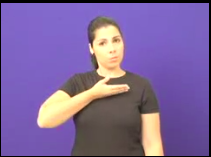
\includegraphics[height=3cm, width=5cm]{src/images/amigo.png}}}%
    \qquad
    \subfloat[Desculpa]{{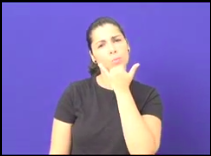
\includegraphics[height=3cm, width=5cm]{src/images/desculpa.png} }}%
    \qquad
    \subfloat[Telefone]{{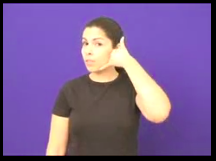
\includegraphics[height=3cm, width=5cm]{src/images/telefone.png} }}%
    \qquad
    \caption{Gestos selecionado para o conjunto de dados}%
    \label{figure:gestos_selecionados}%
    \fonte{Produção do autor} % Adaptado de Dicionário de Libras
\end{figure}

\par Para a aquisição dos dados, foi desenvolvido uma ferramenta (Figura \ref{figure:sistema_aquisicao}) \textit{desktop} multiplataforma na linguagem Python, com o auxílio da biblioteca PyQt, para a criação da interface gráfica e a biblioteca OpenCV, para a manipulação das imagens capturadas.

% Ei!! Problema na imagem, você não declarou ter utilizado o gesto "Idade".... (07/03/2019)
\image{0.60}{image_sistema_aquisicao_de_dados.png}{Tela inicial da aplicação de aquisição de dados}{figure:sistema_aquisicao}{Produção do Autor}

\par Como apresentado na Figura \ref{figure:sistema_aquisicao}, o sistema de aquisição de imagens demonstra exemplos dos gestos que devem ser reproduzidos pelo usuário, uma barra de progresso, e botões para recomeçar a captura ou saber mais sobre o projeto, além da imagem do próprio usuário.

\par Este sistema captura 60 imagens, sendo 20 de cada um dos gestos, em cada uma das imagens capturadas é aplicado uma operação de redimensionamento, isto para que, todas as imagens tenham as dimensões 224x224x3, já que esta é a dimensão aceita pelo \textit{Mobilenet}, o mesmo que será retreinado com os dados que estão sendo coletados. Após a aquisição das 60 imagens o programa cria um arquivo no formato zip e o envia para um \textit{email} criado para o armazenamento dos dados.

\par O programa foi distribuído e ao final houveram 11 colabores, criando assim um conjunto com 660 imagens.

\subsection{Pré-processamento dos dados} 

\par Durante a aquisição das imagens, nenhuma restrição foi emposta aos colaboradores, assim uma etapa de validação de cada uma das imagens teve de ser realizada para garantir que, cada uma das imagens representa o gesto ao qual é indicado, o que resultou na remoção de algumas imagens. A Figura \ref{figure:plot_qtd_apos_filtro} apresenta a relação da quantidade de imagens com cada um dos gestos após a validação realizada.

% Imagem aqui
\image{0.30}{tem_grafico_de_barra.PNG}{Quantidade de imagens por gesto após filtragem}{figure:plot_qtd_apos_filtro}{Produção do Autor}

% Como posso escrever que, isto está sendo feito já que após testes houveram problemas?? Posso escrever aqui mesmo ? ? ?
\par A quantidade de imagens disponíveis após o filtro pode representar problemas para a generalização do modelo, mesmo levando em consideração o retreino que será feito, desta forma será aplicado a técnica de \textit{Data Augmentation}, esta que aumenta a quantidade de imagens realizando modificações com filtros e alterações na base já existente.

\par Neste trabalho, o \textit{Data Augmentation} foi realizado com o auxílio do \textit{Augmentor}, uma biblioteca Python que permite a criação de um \textit{Pipeline} de alterações baseado em probabilidade, assim atribui-se para cada alteração que pode ser aplicada na imagem uma probabilidade de ocorrência, e então o \textit{Augmentor} através destas aplica uma ou várias alterações na base de imagens. A Figura \ref{figure:dataaugmentation} apresenta o código aplicado para esta atividade.

\begin{figure}[H]
    \centering
    \begin{lstlisting}[language=Python]
import Augmentor

p = Augmentor.Pipeline('gestos_editados/treino')

p.flip_left_right(probability=0.6)

p.rotate(probability=0.7, max_left_rotation=3, max_right_rotation=3)
p.rotate(probability=0.4, max_left_rotation=7, max_right_rotation=7)

p.random_distortion(probability=0.5, grid_height=3, grid_width=3, magnitude=2)
p.random_distortion(probability=0.4, grid_height=4, grid_width=4, magnitude=3)

p.skew_left_right(probability=0.3, magnitude=0.7)
p.skew_corner(probability=0.4, magnitude=0.5)

p.shear(probability=0.5, max_shear_left=4, max_shear_right=3)

p.sample(1500)
    \end{lstlisting}
    \caption{\textit{Script} de \textit{Data Augmentation}}
    \label{figure:dataaugmentation}
\end{figure}

\par Veja que, cria-se inicialmente uma instância de \textit{Pipeline} indicando apenas o diretório das imagens de treino, e então todas as possíveis modificações são declaradas na instância de \textit{Pipeline} e junto a cada uma delas uma probabilidade. No fim, é indicado que o total de imagens gerado deve ser 1500.

% Após finalizar esta versão iterar colocando uma tabela com cada operação aplicada no Pipeline, com imagens de exemplo inclusive.. (09/03/2019).

\par Após a aplicação do \textit{Pipeline} o conjunto de treinamento passou a ter 1500 imagens, a Figura \ref{figure:plot_qtd_apos_dataaugmentation} mostra este valor distribuído por gesto.

% Imagem aqui
\image{0.30}{tem_grafico_de_barra.PNG}{Quantidade de imagens por gesto com \textit{Data Aumentation}}{figure:plot_qtd_apos_dataaugmentation}{Produção do Autor}

\subsection{Treinamento da Rede Neural Convolucional}

% Falar sobre o treinamento

\subsection{Distribuição do modelo}

% Posso falar da transformação aqui também...
% Com a finalização do treinamento, o modelo foi salvo inicialmente no formato \textit{h5}, porém para que o mesmo possa ser utilizado fez-se a transformação deste formato para um formato otimizado pela web...(Pegar nome algo assim....).
% Texto explicando para a avó
\par Para tornar a distribuição e utilização da biblioteca simples, foi criado uma \textit{API Rest} para a distribuição do modelo treinado, fazendo com que, os usuários da API não tenham que prover serviços de distribuição dos modelos.....
\par A \textit{API} foi criada utilizando \textit{Flask}, um \textit{microframework} Python para a realização de desenvolvimento web.

% Colocar imagem da página inicial da API... ou mesmo da página de exemplo e tals... Dar valor ao trabalho realizado.

\par O consumo desta \textit{API} é feito através do módulo \textitbf{MobileNetV1Libras} presente na camada \textitbf{Core} do ICan.js.

% Colocar código consumindo o modelo via API aqui....

\subsection{Criação do recurso assistivo}

% Explicando para a avó
\par Após todo o processo de treinamento do modelo de CNN utilizado neste recurso assistivo, foi adicionado na camada \textitbf{Common} da biblioteca o componente \textitbf{Writer}, este que permite a escrita em campos de uma página \textit{web} utilizando gestos de Libras.

% Falar do espaço de tempo....
\par O treinamento da CNN aplicada neste recurso assistivo, como demonstrado, utiliza imagens estáticas, porém para garantir a usabilidade, o método descrito por \citeonline{Magalh2018} é aplicado, desta forma, um conjunto de \textit{frames} é reconhecido pela rede neural e então a média dos resultados é utilizada para a escolha da palavra.

% \par Mesmo o treinamento da CNN aplicado neste recurso assistivo ter sido realizado com imagens estática, o módulo implementado recebe um \textit{stream} de vídeo. Isto porque o usuário define além do \textit{stream} a quantidade de \textit{frames} que deve ser levada em consideração e o tempo entre a aquisição de uma \textit{frame} e outro, fazendo assim com que, a média da classificação destes \textit{frames} seja utilizada como a palavra sendo representada no gesto, assim como apresentado em \cite{Magalh2018}.

\par Toda esta operação da captura de um conjunto de \textit{frames} é feito através de uma função recursiva, demonstrada na Figura \ref{figure:class_recursiva}.

% \par Toda esta operação da captura de \textit{frames} em um intervalo de tempo é feito através de uma função recursiva, demonstrada na Figura \ref{figure:class_recursiva}.

\begin{figure}[H]
    \centering
    \begin{lstlisting}[language=JavaScript]
async function recursiveInterval() {
    try {
        gestures.push(await mobilenetGestures.predictFrame());

        if (gestures.length >= nFrames) {
            // Tira a média de valores classificados
            fnc(getMeanGesture(gestures));
            gestures = [];
        }

        timeout = window.setTimeout(() => {
            recursiveInterval();
        }, delay * 1000);       
    } catch(err) {
        if (timeout !== null) {
            window.clearTimeout(timeout);
        }

        console.error("librasWriter", err);
    }
}
    \end{lstlisting}
    \caption{\textit{Script} de classificação recursiva}
    \label{figure:class_recursiva}
\end{figure}

% Explicação para a avó
% Na explicação final, não deixe de colocar explicações levando em consideração o código (Trechos e números de linhas).....
\par Veja que, a cada vez chamada a função recursiva, é feita uma classificação, e seu resultado é inserido em uma lista, após isto a quantidade de elementos dentro da lista é verificado, caso seja igual ou maior ao limite definido pelo usuário, é feito a média das classificações e então o resultado é devolvido ao usuário, caso contrário a função fica parada por um intervalo de tempo, definido pelo usuário e então após o intervalo a função é chamada novamente, repetindo todo o ciclo.

\section{Controle de \textit{mouse} com movimentos da cabeça}

\par Este recurso assistivo permite a interação de usuários com deficiência motora a navegação de páginas da \textit{web} com movimentos da cabeça.

\par O desenvolvimento deste recurso assistivo ocorreu através da utilização do modelo PoseNet junto a regressão linear.

% % Explicação para a avó
% \par Para isto o modelo identifica os pontos do corpo do usuário, os valores da posição do ponto identificado é aplicado em uma regressão, esta que devolve a posição a qual o usuário está  

\subsection{Mapeamento dos movimentos}

% Ao descrever melhor o mapeamento, dar mais enfâse para certas partes do código... Como a de classificação do PoseNet, já que houve um trabalho para a criação deste código....

% Explicação para a avó
\par O mapeamento dos movimentos do usuário para movimentos do mouse é feito através da integração do PoseNet e de regressão linear, como já explicado anteriormente.

\par Para este desenvolvimento, utilizou-se os conceitos apresentados por \cite{Papoutsaki2016}, onde o mapeamento dos gestos era feito utilizando diferentes modelos de regressão, porém neste trabalho utilizou-se apenas a regressão linear, e o método de identificação dos pontos do usuário, neste caso foi o PoseNet.

\par Com isto, há um módulo dentro do \textitbf{Core} da biblioteca nomeado PoseNet, que possui os mecanismos de utilização do PoseNet já implementado no TFJS. 

\par Desta forma, a saída da identificação do PoseNet, ou seja, a posição onde está a parte do corpo interessada, neste caso o nariz, passa como entrada para a regressão, que foi previamente calibrada para mapear a posição do mouse com a posição do nariz do usuário, desta forma é feita a predição da posição onde o usuário pode estar apontando o nariz.

\par Para as representações de regressão, dentro do \textitbf{Core} há o módulo \textitbf{Regression}, que possui as regressões.

% Mostrar código....

\subsection{Calibração da regressão}

\par Foi especificado que, utiliza-se de regressões para o mapeamento após a identificação feita com o PoseNet, porém estes modelos precisam de alguma forma serem calibrados e assim se ajustar as possibilidades de movimentação de cada usuário, para facilitar este processo de calibração o ICan.js fornece uma \textit{API} de calibração, esta presente na camada \textitbf{Core}.

% Colocar imagens...

% Imagem mostrando como funciona todo o processo...

% Veja que na figura acima

% Um dos grandes desafios do desenvolvimento dos recursos assistivos para deficientes auditivos foi a base de dados, isto porque o que tange o conhecimento do autor, não há nenhuma base de dados de imagens de sinais da Língua Brasileira de Sinais disponível publicamente, de modo a ser necessário a criação de uma base de dados própria.

% \par A especificação e desenvolvimento de cada uma das camadas será feita nas seções a frente.



% \subsection{Camada Core}

% A camada \textitbf{Core} da biblioteca ICan.js é responsável pelas principais funcionalidades

% \par Como apresentado na Figura \ref{figure:icanjsarch}, a camada \textitbf{Core} disponibiliza funcionalidades essenciais para a criação de recursos assistivos, com por exemplo, os modelos de rede neural e regressão, assim como facilidades para acesso e manipulação da \textit{webcam} do usuário. Por outro lado, a camada \textitbf{Common} apresenta funcionalidades de alto nível criadas utilizando o \textitbf{Core}, como por exemplo as funcionalidades de controle de \textit{mouse} através de movimentos com a cabeça, e transcrição de gestos de Libras para texto.

% \par As subseções a frente apresentam 


% % (23/02/2019) -> Talvez aplicar O NVIDIA Digits para demonstrar algumas coisas da rede, formas de identificação....Alguma coisa assim.... 

% % Colocar algum texto desta forma como está abaixo, ou algo assim....
% % Este capítulo apresenta os recursos assistivos que foram desenvolvidos durante a criação deste trabalho, como forma de confirmação dos estudos de casos levantados 
% % Este capítulo apresenta os processos de coleta e pré-processamento dos dados, treinamento e validação da CNN e o desenvolvimento da biblioteca ICan.js.

% % Conversando com Giuliano hoje (07/03/2019), ele me recomendou criar uma seção para falar sobre a biblioteca, e depois falo dos recursos assistivos que foram desenvolvidos e incorporados dentro da biblioteca. 
% \section{Estrutura da Biblioteca}

% \par 

% % Aqui será descrito sobre a biblioteca, como ela foi dividida, para assim justificar a apresentação dos demais conteúdos abaixo....

% % Será que neste capítulo é legal separar ?? Ou ficaria um lixo ? (01/02/2019)
% % Sabe, separar entre as aplicações que eu fiz.... (01/02/2019)
% %% R: Falei com o Lipe, ele disse que acha interessante (02/02/2019)

% % Outra questão, onde colocar que tudo isto foi unificado através de uma biblioteca, um módulo.... ? ? ?


% \section{Recurso assistivo para deficientes auditivos}

% % Veja que, o que será escrito aqui, facilita ao leitor entender o problema que está sendo resolvido...

% % O recursos assistivo desenvolvido, como protótipo, para ajudar aos deficiêntes auditivos foi uma ferramenta capaz de permitir a escrita de textos em páginas da web através de gestos de Libras, as seções seguintes demonstram as etapas adotadas para o desenvolvimento desta ferramenta.

% \subsection{Aquisição dos dados}

% % Caso eu consiga demonstrar que a coisa ficou interessante, vale colocar o pq a base de dados foi coletada assim ? Sem grandes restrições ????
% \par Um dos grandes desafios do desenvolvimento dos recursos assistivos para deficientes auditivos foi a base de dados, isto porque o que tange o conhecimento do autor, não há nenhuma base de dados de imagens de sinais da Língua Brasileira de Sinais disponível publicamente, de modo a ser necessário a criação de uma base de dados própria.

% % Aqui utilizeo como base o trabalho do Ilharco...Lá ele disse que fez a escolha junto a associação de Apoio ao Deficiente Auditivo....
% % Caso falem algo....beleza, fala com a associação.......
%  % Colocar referências aqui, isto ajuda muito
% \par Para este trabalho, foram escolhidos gestos que podem ser classificados com apenas um \textit{frame}, sendo eles (a) Amigo, (b) Desculpa, (c) Telefone. A Figura \ref{figure:gestos_selecionados} apresenta cada um destes gestos.

% \begin{figure}[H]%
%     \centering
%     \subfloat[Amigo]{{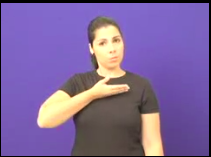
\includegraphics[height=3cm, width=5cm]{src/images/amigo.png}}}%
%     \qquad
%     \subfloat[Desculpa]{{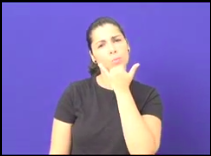
\includegraphics[height=3cm, width=5cm]{src/images/desculpa.png} }}%
%     \qquad
%     \subfloat[Telefone]{{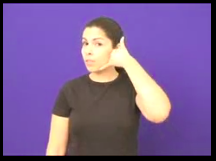
\includegraphics[height=3cm, width=5cm]{src/images/telefone.png} }}%
%     \qquad
%     \caption{Gestos selecionado para o conjunto de dados}%
%     \label{figure:gestos_selecionados}%
%     \fonte{Produção do autor} % Adaptado de Dicionário de Libras
% \end{figure}

% % Devo falar mais sobre a aplicação ?? (05/03/2019)
% \par A aquisição dos dados foi feita através de uma aplicação desenvolvida em Python (Figura \ref{figure:tela_inicial}) junto a biblioteca de criação de interfaces gráficas PyQt e a biblioteca de visão computacional OpenCV \cite{opencv2019}. Esta aplicação através da \textit{webcam} do usuário, adquire 60 imagens, sendo 20 de cada um dos gestos selecionados. Após a aquisição, as imagens são redimensionadas pela aplicação, para um formato 224x224x3 e então envia os arquivos das imagens por \textit{email}. O processo de redimensionamento é feito pois o algoritmo de treinamento da CNN recebe como entrada imagens no formato 224x224x3.

% % Ei!! Problema na imagem, você não declarou ter utilizado o gesto "Idade".... (07/03/2019)
% \image{0.60}{image_sistema_aquisicao_de_dados.png}{Tela inicial da aplicação de aquisição de dados}{figure:tela_inicial}{Produção do Autor}

% % Descrever que, foram onze colaboradores, porém foram utilizados dados de apenas 10 para o treinamento e 11 para o teste...
% % Assim deixo a coisa justa ao apresentar a matriz de confusão
% \par A aplicação foi distribuída para vários usuários e no total houveram onze colaboradores, com isto um total de 660 imagens foram coletadas, distribuídas igualmente entre todos os gestos.

% \subsection{Pré-processamento dos dados} 
% % Neste tópico acho que ainda está pouco claro o que foi feito... Rever depois, adicionando mais detalhes e imagens =D

% % Perguntar ao Sr. Claudio se a seleção de imagens boas e ruins entra no pré-processamento dos dados...
% % 07/03/2019 -> Falei com o Sr. Cláudio, e ele disse que está mesmo para pré-processamento...

% \par Após realizar a aquisição das imagens, cada uma delas foi avaliada para garantir que os gestos haviam sido feitos corretamente pelos colaboradores. Nesta etapa algumas imagens foram removidas do conjunto. A Figura (TTTY) apresenta a relação da quantidade de imagem com cada um dos gestos após a validação realizada.

% % ToDo: Criar o plot com a quantidade de imagens e os gestos....
% % Os dados: (Teste + Treino)
% %   - Amigo: 38 + 168
% %   - Desculpa: 19 + 160
% %   - Telefone: 38 + 151
% % Total: 574

% % ToDo: Criar parágrafo para falar sobre a divisão dos dados
% \par Com a validação do conjunto de dados realizada, o mesmo foi dividido em dados de treino e dados de teste, como forma de facilitar a validação da RNA, assim como citado anteriormente. Para este caso, um \textit{script} feito em Python (Figura \ref{figure:script_separacao_dados}), com o auxilio da biblioteca \textit{sklearn}, foi criado para separar os dados, de forma randômica, utilizando 80\% para o conjunto de treino e 20\% para o teste.

% % Preciso colocar o source do `move_data` ?
% \begin{figure}[H]
%     \centering
%     \begin{lstlisting}[language=Python]
% import os
% import numpy as np

% from shutil import copyfile

% from sklearn.model_selection import train_test_split

% x, y = [], []

% for root_dir in os.listdir():
%     files = os.listdir(root_dir)

%     x.extend(files)
%     y.extend(np.repeat(root_dir, len(files)))

% x_train, x_test, y_train, y_test = train_test_split(x, y, \ test_size=0.20, random_state=992)

% move_dados(x_train, y_train, 'treino')
% move_dados(x_test, y_test, 'teste')

%     \end{lstlisting}
%     \caption{\textit{Script} para separar os dados de treino e teste}
%     \label{figure:script_separacao_dados}
% \end{figure}

% % Colocar alguma referência no Data Augmentation...
% % Mudar isto, talvez falar apenas que é um conjunto pequeno....
% \par O conjunto de dados adquiridos para o trabalho não é considerado grande, já que podem haver muitas variações principalmente no cenário e vestuário dos usuários, desta forma ao realizar a divisão, o conjunto utilizado no treino fica ainda menor, podendo haver problemas relacionados a \textit{Overfitting}. Para resolver este problema, foi aplicado a técnica de \textit{Data Augmentation}, que de acordo com \citeonline{Amidi2018Tricks} pode ser utilizado quando há conjuntos pequenos de dados para o treinamento de CNNs. Nesta técnica, imagens artificiais são criadas a partir do conjunto de testes, isto feito através da aplicação de filtros e distorções na imagem \cite{Amidi2018Tricks}.

% % Colocar o porque estas transformações foram escolhidas, acho que não.....
% Neste trabalho foi utilizado um \textit{Pipeline} de \textit{Data Augmentation} probabilístico, onde para cada filtro ou distorção há uma probabilidade de ser aplicado na imagem, no total 1500 imagens das três classes foram geradas. O \textit{script} foi criado em Python, e é apresentado na Figura \ref{figure:dataaugmentation}.

% \begin{figure}[H]
%     \centering
%     \begin{lstlisting}[language=Python]
% import Augmentor

% p = Augmentor.Pipeline('gestos_editados/treino')

% p.flip_left_right(probability=0.6)

% p.rotate(probability=0.7, max_left_rotation=3, max_right_rotation=3)
% p.rotate(probability=0.4, max_left_rotation=7, max_right_rotation=7)

% p.random_distortion(probability=0.5, grid_height=3, grid_width=3, magnitude=2)
% p.random_distortion(probability=0.4, grid_height=4, grid_width=4, magnitude=3)

% p.skew_left_right(probability=0.3, magnitude=0.7)
% p.skew_corner(probability=0.4, magnitude=0.5)

% p.shear(probability=0.5, max_shear_left=4, max_shear_right=3)

% p.sample(1500)
%     \end{lstlisting}
%     \caption{\textit{Script} para separar os dados de treino e teste}
%     \label{figure:dataaugmentation}
% \end{figure}

% % Sobre os dados do data augmentation
% %   - Amigo: 502
% %   - Desculpa: 524
% %   - Telefone: 474
% % Total: 1500

% % ToDo: Colocar exemplos de imagens geradas no Augmentation...
% % ToDo: Colocar as quantidades de imagem após o Data Augmentation...

% \subsection{Treinamento da Rede Neural Artificial}

% % ToDo: Falar sobre o retreino do Mobilenet
% %% Posso utilizar como base a exposição feita pelo Felipe....
% % ToDo: Falar sobre a exportação do modelo para o formato web...

% \subsection{Distribuição do modelo}

% % ToDo: O foco deste trabalho é aplicar o Deep Learning nas tecnologias Web, para isto uma API foi criada para a distribuição dos modelos utilizados na biblioteca.....
% % ToDo: Falar do Flask.
% % Rotas...
% % Código básico da API

% \section{Recurso assistivo para deficiência motora}

% % Estou em dúvidas sobre o que colocar aqui...

% % Falar que utilizei o trabalho do WebGazer como base, porém toda a identificação é feita utilizando o PoseNet....
% % Terá de fazer comparações ao Webgazer.js ? ? ? Acho que não, são coisas diferentes....
% % Falar sobre o OJ Ramos ??? Acho que sim...... Falar que ele gerou um produto com isto.....

% \subsection{Calibração}

% % ToDo: Falar sobre a API de calibração...

% ---

% ---
% Incluindo Capitulo 4 - Casos de Testes
\newpage
\chapter{Resultados}

\par Neste capítulo serão apresentados os resultados do modelo gerado e as páginas \textit{web} criadas para testar os módulos implementados no ICan.js

\section{Tradução de Libras para texto}

\par Nesta seção, os resultados obtidos com a tranferência de aprendizado realizada no modelo \textit{MobileNet} e também das páginas de testes deste recurso assistivo.

\subsection{Resultados da transferência de aprendizado do modelo \textit{MobileNet}}

\image{0.23}{resultados/resultados_rede_neural.jpg}{Resultado do retreino do \textit{MobileNet}}{figure:historico_retreino}{Produção do Autor}

\par A Figura \ref{figure:historico_retreino} mostra a acurácia e a perda do modelo durante seu retreino, nota-se que, o processo de retreino levou 5 épocas para atingir bons resultados, isto, tanto na diminuição da perda, quanto no aumento da acurácia do modelo, que nos dois casos, nas primeiras épocas não estavam apresentando bons resultados.

\par O comportamento dos resultados na Figura \ref{figure:historico_retreino}, onde, mesmo os dados de treino sendo 100\% identificados a partir da segunda época e tendo poucas perdas, mas, para os dados de teste, tem-se uma variação inversamente proporcional entre a crescente da acurácia e a diminuição da perda. 

\par Para avaliar o desempenho do modelo, além dos resultados da Figura \ref{figure:historico_retreino}, fez-se a utilização da matriz de confusão, esta que vincula as classes esperadas com a preditas em cada um dos valores presentes nos dados. Como citado anteriormente, os dados foram separados em dois conjuntos, o primeiro para treino/teste e o segundo para validação, isto para garantir que, o modelo gerado de nenhuma forma possui bons resultados somente por conta de um viés aos dados. Desta forma, duas matrizes de confusão foram criadas, uma para o conjunto de treino e teste (Figura \ref{figure:matriz_confusao_teste}) e outra para o conjunto de validação (Figura \ref{figure:matriz_confusao_validacao}).

\par A matriz de confusão da Figura \ref{figure:matriz_confusao_teste}, utilizou apenas os dados de teste, e mesmo nestes havendo imagens de participantes que foram apresentados ao modelo nos dados de treino, uma pequena quantidade de erro foi registrada nas classes Amigo e Desculpa.

\image{0.60}{resultados/matriz_de_confusao_teste.png}{Matriz de confusão do modelo \textit{MobileNet} retreinado com dados de teste}{figure:matriz_confusao_teste}{Produção do Autor}

\par Já na matriz de confusão de validação (Figura \ref{figure:matriz_confusao_validacao}), que possui dados nunca antes apresentados para o modelo retreinado apresentou excelentes resultados, não errando em nenhuma das classes.

\image{0.60}{resultados/matriz_de_confusao_validacao.png}{Matriz de confusão do modelo \textit{MobileNet} retreinado com dados de validação}{figure:matriz_confusao_validacao}{Produção do Autor}

\par É interessante notar que, o erro pode ter ocorrido para a matriz dos dados de teste (Figura \ref{figure:matriz_confusao_teste}) por conta de dados que, mesmo sendo filtrados, apresentam características muito diferentes das levadas em consideração pelo modelo, o que acaba não ocorrendo nos dados do conjunto de validação (Figura \ref{figure:matriz_confusao_validacao}).

\subsection{Aplicação do recurso assistivo desenvolvido}

\par Além da validação realizada nos resultados do \textit{MobileNet} utilizado neste recurso assistivo, uma aplicação\footnote{Disponível em: \url{https://icanjs-examples.netlify.com/escrita-de-texto/}} foi desenvolvida para validar a eficácia da biblioteca na distribuição de um recurso assistivo que permite a escrita de textos em campos de páginas \textit{web}. Nesta aplicação espera-se que a biblioteca permita a escrita através de Libras em um campo de uma página \textit{web}.

\subsubsection{Página inicial}

\par Esta aplicação possui apenas uma página, em seu início (Figura \ref{figure:case_libras_1}), há uma descrição dos objetivos da página e também sobre o projeto desenvolvido.

\image{0.70}{resultados/estudo-de-caso_escrita-de-texto/1.PNG}{Primeira parte da página da aplicação desenvolvido}{figure:case_libras_1}{Produção do Autor}   

\par Após a parte de apresentação, há uma seção que explica as formas de funcionamento (Figura \ref{figure:case_libras_2}) do exemplo, nesta são descritas as duas formas de funcionamento descritas durante o Capítulo \ref{ch:desenvolvimento}, a primeira (Exclusiva) transcrevendo o gesto capturado em cada \textit{frame} e a segunda (Contínua), que considera os \textit{frames} capturados em um intervalo de tempo para definir o gesto que deve ser transcrito.

\image{0.70}{resultados/estudo-de-caso_escrita-de-texto/2.PNG}{Seção de explicações sobre o funcionamento do exemplo da aplicação}{figure:case_libras_2}{Produção do Autor}   

\par Com o final das explicações o exemplo presente na aplicação é apresentado, disponibilizando as duas formas de funcionamento explicadas na Figura \ref{figure:case_libras_2}. A primeira forma de funcionamento não permite a geração de um texto contínuo, transcrevendo gesto a gesto para o campo da página (Figura \ref{figure:case_libras_3_1}). 

\image{0.60}{resultados/estudo-de-caso_escrita-de-texto/3_1.PNG}{Exemplo de funcionamento exclusivo}{figure:case_libras_3_1}{Produção do Autor} 

\par Já a segunda forma de funcionamento, presente na Figura \ref{figure:case_libras_3_2}, permite a escrita de textos contínuos, utilizando intervalos de tempo, o que também deixa seu uso agradável.

\image{0.60}{resultados/estudo-de-caso_escrita-de-texto/3_2.PNG}{Exemplo de funcionamento contínuo}{figure:case_libras_3_2}{Produção do Autor} 

\par Com isto, o objetivo da escrita de textos com Libras foi atingido através do módulo implementado na biblioteca.

\section{Controle do \textit{cursor} do \textit{mouse} com movimentos da cabeça}

\par Esta seção apresenta a aplicação criada com os resultados obtidos na implementação do ICan.js e suas funcionalidades para o recurso assistivo de controle de \textit{cursor}.

\subsection{Aplicação do recurso assistivo desenvolvido}

\par Para realizar testes com o recurso assistivo implementado na biblioteca, fez-se a criação de uma aplicação\footnote{Disponível em: \url{https://icanjs-examples.netlify.com/controle-de-mouse/}}que consome os recursos da biblioteca. Nas subseções abaixo as páginas desenvolvidas serão apresentadas.

\subsubsection{Página inicial e calibração}

\par A página inicial da aplicação desenvolvida possui informações gerais do projeto e também da forma de funcionamento do mesmo, como exibido na Figura \ref{figure:case_cursor_tela_1}.

\image{0.47}{resultados/estudo-de-dado_controle-de-cursor/controle_do_mouse_1.PNG}{Tela inicial}{figure:case_cursor_tela_1}{Produção do Autor}

\par Na Figura \ref{figure:case_cursor_tela_1}, logo após a explicação do exemplo de execução da aplicação há um botão para que a execução seja iniciada, no momento em que o usuário clica neste a tela de calibração do modelo de regressão que será utilizado é exibida (Figura \ref{figure:case_cursor_tela_2}), nesta primeira tela de calibração, informações gerais são exibidas e então o usuário pode começar a calibração.

\image{0.40}{resultados/estudo-de-dado_controle-de-cursor/controle_do_mouse_2.PNG}{Tela inicial de calibração}{figure:case_cursor_tela_2}{Produção do Autor}

\par Com o usuário iniciando a aplicação, fica disponível para ele uma matriz 3X3 que ao ser clicada, salva a posição do \textit{cursor} e também do nariz do usuário. Aqui é esperado que, quando o usuário clicar nos pontos da matriz ele esteja apontando o nariz para a direção do ponto. Cada clique válido do usuário, faz uma barra de progresso no topo da tela ser atualizada (Figura \ref{figure:case_cursor_tela_2_2}).

\image{0.33}{resultados/estudo-de-dado_controle-de-cursor/controle_do_mouse_2_2.PNG}{Matriz de calibração e barra de progresso}{figure:case_cursor_tela_2_2}{Produção do Autor}

\par Ao término da coleta de pontos, o modelo é calibrado e salvo no \textit{sessionStorage}\footnote{Local para armazenamento temporário em navegadores} do navegador, ao mesmo tempo que, uma mensagem de finalização é exibida (Figura \ref{figure:case_cursor_tela_2_3}), nesta mensagem o usuário pode escolher continuar para a próxima tela ou mesmo recalibrar o modelo, sendo que, ao clicar nesta segunda opção, o processo visto anteriormente é recomeçado.

\image{0.40}{resultados/estudo-de-dado_controle-de-cursor/controle_do_mouse_2_3.PNG}{Aviso da finalização da calibração}{figure:case_cursor_tela_2_3}{Produção do Autor}

% \subsubsubsection{Geração dos regressores}

% \par No momento em que a calibração é realizada, dois modelos são gerados, como descrito no Capítulo \ref{ch:desenvolvimento}, a forma do ajuste feito por cada um destes modelos é exibida na Figura \ref{figure:modelos_calibrados}.

% \image{0.60}{recurso_assistivo_controle_do_mouse/plot_modelo.png}{Modelos de regressão gerados durante a calibração}{figure:modelos_calibrados}{Produção do Autor}

\subsubsection{Páginas de exemplos}

\par Com a finalização da calibração é exibido ao usuário uma página para seleção de exemplos (Figura \ref{figure:case_cursor_tela_3}), nesta está disponível uma página para testar a funcionalidade de \textit{scrolling} de páginas, isto feito através da leitura de um texto e outra para desenhar, que aproveita os recursos da camada \textit{Core} para construir uma aplicação de desenhos através de gestos.

\image{0.47}{resultados/estudo-de-dado_controle-de-cursor/controle_do_mouse_3.PNG}{Página de seleção de exemplos}{figure:case_cursor_tela_3}{Produção do Autor}

\par A página de leitura de texto (Figura \ref{figure:case_cursor_tela_4}) utiliza a função \textit{screenScroller}, sem nenhuma mudança, o resultado é uma \textit{div} que representa o \textit{cursor} criado que é movimentado através dos gestos.

\image{0.47}{resultados/estudo-de-dado_controle-de-cursor/controle_do_mouse_4.PNG}{Página de leitura de texto com a função \textit{screenScroller}}{figure:case_cursor_tela_4}{Produção do Autor}

\par Já na página de desenho, foi criado uma nova forma de aplicação das funcionalidades presentes do ICan.js, presentes na camada \textit{Core}, demonstrando que, além dos recursos já implementados na camada \textit{Common} é possível realizar a implementação de novas funcionalidades com a biblioteca.

\image{0.47}{resultados/estudo-de-dado_controle-de-cursor/controle_do_mouse_5.PNG}{Canvas de desenho criado no exemplo de desenho com o ICan.js}{figure:case_cursor_tela_5}{Produção do Autor}

\par Com isto, o objetivo da criação de um recurso assistivo para controle de \textit{cursor} com gestos do usuário foi atingido através das funcionalidades implementadas no ICan.js.

% \section{Experimentos}

% \par \textbf{O ORIENTADOR DISSE QUE, DA MESMA FORMA COMO FOI FEITO NA CAPÍTULO 3, A DIVISÃO PODE SER FEITA AQUI TAMBÉM! =D}

%% ?? ? ? ?
% Ainda estou com dúvida sobre como apresentar os resultados...

% Devo apresentar os resultados separado da mesma forma que o capítulo de desenvolvimento ? Ou posso fazer algo como demonstrar os resultados da rede, e então já a implementação da biblioteca, junto aos exemplos....

% ---

% ---
% Incluindo Capitulo 5 - Conclusao
\newpage
\chapter{Considerações Finais}

\par Neste capítulo as contribuições e conclusões deste Trabalho são apresentadas, assim como as publicações e os trabalhos futuros.

\section{Contribuições e conclusões}

\par As contribuições apresentadas neste trabalho são:

\begin{enumerate}
    \item Um modelo de RNC criado sob o \textit{MobileNet} capaz de classificar gestos de Libras;
    \item Integração do funcionamento de dois algoritmos para a produção de predições; 
    \item Biblioteca JavaScript que fornece recursos assistivos desenvolvidos com técnicas de Aprendizado Profundo.
\end{enumerate}

\par Neste trabalho foi apresentado uma biblioteca para a linguagem JavaScript que fornece dois recursos assistivos, o controle de \textit{cursor} através de movimentos com a cabeça e a escrita de texto em campos com gestos de Libras, ambos para ambiente \textit{web}.

\par Para o desenvolvimento do recurso assistivo de controle de \textit{cursor} foram utilizados o modelo de RNC PoseNet junto a regressões lineares, o que mesmo dependendo de uma calibração permitiu aos usuários a navegação dentro de uma página sem a necessidade de utilizar um \textit{mouse}.

\par No desenvolvimento do recurso assistivo de escritas com sinais de Libras fez-se a utilização do MobileNet com a técnica de aprendizado por transferência no treinamento, que utilizou um conjunto de dados criados neste trabalho. A métrica utilizada para a avaliação foi a matriz de confusão, que demonstrou que o modelo apresentou bons resultados, tanto no treino e teste quanto na validação.

\par Todas as funcionalidades e o ecossistema criado para o desenvolvimento do ICan.js junto aos recursos assistivos citados anteriormente podem ser utilizado como base para a criação de outros recursos assistivos, e ainda, a forma de implementação da biblioteca e as técnicas utilizadas nela permitiram a criação de recursos assistivos mais acessíveis, que para serem utilizados dependem exclusivamente de tecnologias já presentes no dia-a-dia das pessoas, não sendo necessário a aquisição de nenhum \textit{hardware} ou \textit{software} específico.

\subsection{Publicações}

\par Como resultado deste trabalho foram publicados os seguintes artigos em periódicos:

\begin{enumerate}
    \item \textit{Deep Learning} aplicado na conversão de Libras em texto - \cite{fmenino2019a};
    \item Uso de \textit{Deep Learning} para desenvolver tecnologias assistivas de baixo custo - \cite{fmenino2019b}.
\end{enumerate}

\section{Trabalhos futuros}

Os resultados deste trabalho não encerram as pesquisas sobre recursos assistivos na \textit{web} utilizando técnicas de Aprendizado Profundo, mas abrem oportunidades para os seguintes trabalhos futuros:

\begin{itemize}
    \item Adicionar outros modelos de regressão;
    \item Implementar método que permita ao usuário clicar na tela no recurso assistivo de controle de \textit{cursor};
    \item Melhorar a movimentação do \textit{cursor} com predições extras, estas relacionadas aos locais onde o usuário deseja alcançar na tela;
    \item Aumentar a quantidade de gestos de Libras disponíveis no ICan.js;
    \item Incrementar os pontos de referência para a movimentação do \textit{cursor}.
\end{itemize}

% ---

% ---
% Referências bibliográficas
\bibliography{ref/referencias}
% ---
\end{document}
